\documentclass[12pt,onecolumn,a4paper,twoside]{article}
\usepackage[T1]{fontenc}
\usepackage{textcomp}
\usepackage[utf8x]{inputenc}
\usepackage[english,greek]{babel}
\usepackage{amsmath,amsfonts,amssymb}
% \usepackage{mathtools}
\usepackage[square, numbers, comma, sort]{natbib}
% \usepackage{fullpage}
\usepackage{a4wide}
\usepackage[version=3]{mhchem}
\usepackage{kerkis}
%\usepackage{gfsartemisia-euler}
%\usepackage{gfsartemisia}
%\usepackage{gfsdidot}
\renewcommand*\ttdefault{cmtt}
\usepackage{eulervm}
\usepackage{verbatim}
\usepackage{color}
\usepackage{gensymb}
\usepackage[colorlinks=true]{hyperref}
\usepackage{graphicx}
\usepackage{wrapfig}
\usepackage{float}
\usepackage{rotating}
\usepackage{longtable}
% for frontpage
\usepackage{adjustbox}
\usepackage[normalem]{ulem}
% figures, custom commands
\usepackage[hang,small,it]{caption}
\usepackage{subcaption}
\captionsetup{figurename=Σχήμα}
\newcommand{\eng}[1]{\selectlanguage{english}#1\selectlanguage{greek}}
\newcommand{\gre}[1]{\selectlanguage{greek}#1\selectlanguage{english}}
\newcommand{\ttt}[1]{\selectlanguage{english}\texttt{#1}\selectlanguage{greek}}
\newcommand{\itcaption}[2][]{\caption[#1]{\textit{#2}}}
\newcommand{\rmcaption}[2][]{\caption[#1]{#2}}
\newcommand{\norm}[1]{\lVert#1\rVert}
\renewcommand{\vec}[1]{\mathbf{#1}} \let\oldhat\hat
\renewcommand{\hat}[1]{\oldhat{\mathbf{#1}}}

\begin{document}
\pagenumbering{roman}
\adjustbox{valign=t}{
  \begin{minipage}{0.14\linewidth}
    
\includegraphics[height=2cm, keepaspectratio=true]{figures/upatras-logo.jpg}
  \end{minipage}}\hfill
\adjustbox{valign=t}{\begin{minipage}[t]{0.76\linewidth}
    {\Large\textsc{\textbf{Πανεπιστημιο Πατρων}}}\\[5pt]
    {\textsc{Τμημα Ηλεκτρολογων Μηχανικων Και Τεχνολογιας Υπολογιστων\\
        Τομεας Τηλεπικοινωνιων Και Τεχνολογιας Πληροφοριας\\
        Εργαστηριο Απεικονισης Πληροφοριας Kαι Εικονικης Πραγματικοτητας\\}}
  \end{minipage}}
\noindent\makebox[\textwidth]{\rule{\textwidth}{0.4pt}}

\large
\vspace{1.5cm}
\begin{center}
  {\huge \textsc{\textbf{Διπλωματικη Εργασια}}}\\[1cm]
  του φοιτητή του Τμήματος Ηλεκτρολόγων Μηχανικών και Τεχνολογίας Υπολογιστών\\
  της Πολυτεχνικής Σχολής του Πανεπιστημίου Πατρών\\[2cm]
  \textsc{\Large Σπαθη-Παπαδιωτη Αριστοτελη του Γερασιμου}\\[10pt]
  \textsc{Αριθμος Μητρωου: $7729$}\\[1.5cm]
  \uline{Θέμα}\\[0.3cm]
  \textbf{\Large Προσομοίωση πρόσπτωσης τσουνάμι σε ακτογραμμή}\\[1.2cm]
  \uline{Επιβλέπων}\\[0.3cm]
  \textsc{\Large Μουστακας Κωνσταντινος}\\[0.8cm]
  \textbf{Αριθμός Διπλωματικής Εργασίας:}\\
  \vfill Πάτρα, Δεκέμβριος 2015
\end{center}
\thispagestyle{empty}

\newpage\null\thispagestyle{empty}\newpage

\large
\begin{center}
  {\huge \textsc{ΠΙΣΤΟΠΟΙΗΣΗ}}\\[1cm]
  Πιστοποιείται ότι η Διπλωματική Εργασία με θέμα\\[0.5cm]
  \textbf{\Large Προσομοίωση πρόσπτωσης τσουνάμι σε ακτογραμμή}\\[1cm]
  Του φοιτητή του Τμήματος Ηλεκτρολόγων Μηχανικών και Τεχνολογίας Υπολογιστών\\[0.5cm]
  \textsc{\Large Σπαθη-Παπαδιωτη Αριστοτελη του Γερασιμου}\\[10pt]
  Αριθμός Μητρώου: $7729$\\[2cm]
  Παρουσιάστηκε δημόσια και εξετάστηκε\\στο Τμήμα Ηλεκτρολόγων Μηχανικών και
  Τεχνολογίας Υπολογιστών στις\\[0.5cm]
  ......../......../................\\
\end{center}

\vfill
\begin{minipage}[t]{0.5\textwidth}
  \begin{flushleft}
    Ο Επιβλέπων\\
    Επίκουρος Καθηγητής\\
    Μουστάκας Κωνσταντίνος
  \end{flushleft}
\end{minipage}
\begin{minipage}[t]{0.5\textwidth}
  \begin{flushright}
    Ο Διευθυντής του Τομέα\\
    Καθηγητής Φακωτάκης Νίκος
  \end{flushright}
\end{minipage}
\thispagestyle{empty}
\normalsize
\newpage

%%% Local Variables:
%%% mode: latex
%%% TeX-master: "report"
%%% End:

\cleardoublepage
\linespread{1.3}
% \begin{minipage}[t][0.49\textheight][t]{\textwidth}
\section*{Περίληψη}
\paragraph{} Αντικείμενο της παρούσας εργασίας ήταν η προσομοίωση της πρόσ\-πτω\-σης ενός
τσουνάμι σε ακτογραμμή πόλης. Έμφαση δόθηκε στη διατήρηση της ορμής, καθώς η κατανομή της
στο χώρο και το χρόνο είναι καθοριστική για τις επιπτώσεις του κύματος στην
ακτογραμμή. Για το λόγο αυτό, υιοθετήθηκε μια υβριδική μέθοδος προσομοίωσης, βασισμένη στη
μέθοδο \eng{Smoothed Particle Hydrodynamics} (\eng{SPH}), εμπλουτισμένη όμως με
γεωμετρικούς περιορισμούς και αλληλεπιδράσεις υλικών σωμάτων. Η υλοποίηση είναι αποτέλεσμα
της συνεργασίας της μηχανής φυσικής \eng{Bullet} και μιας μηχανής \eng{SPH}, που
επεξεργάζονται αλληλοδιάδοχα την δυναμική κατάσταση του ρευστού σε κάθε χρονικό
βήμα. Επιπλέον, για την καλύτερη απόδοση της προσομοίωσης αναπτύχθηκε ειδική δομή
δεδομένων (\eng{LP grid}) για τη διατήρηση της τοπικότητας κατά την αποθήκευση των
δεδομένων στη μνήμη και της ελαχιστοποίησης του χρόνου πρόσβασης σε αυτά. Τα δεδομένα της
προσομοίωσης εξάγονται σε ειδικής μορφής αρχεία κειμένου (\eng{VTK}), επιτρέποντας την εκ
των υστέρων διαδραστική οπτικοποίηση και επεξεργασία. Πειραματικά αποτελέσματα δείχνουν τα
πλεονεκτήματα της καταγραφής ώσεων για εκτίμηση πιθανής καταστροφής και την αξιολόγηση
στρατηγικών προστασίας.

\paragraph{Λέξεις Κλειδιά} Προσομοίωση ρευστών, τσουνάμι, \eng{SPH}, αλληλεπίδραση
τσουνάμι-α\-κτο\-γραμ\-μής, οπτικοποίηση δυνάμεων
% \end{minipage}
\clearpage
% \begin{minipage}[b][0.49\textheight][t]{\textwidth}
\selectlanguage{english}
\section*{Abstract}
\paragraph{} The objective of this thesis was the simulation of a tsunami impact upon an
urban coastline. Emphasis was given to the conservation of momentum, as its distribution
in space and time is the main factor of the wave's effects on the coastline. Due to this,
a hybrid simulation method was adopted, based on the Smoothed Particle Hydrodynamics (SPH)
method, enriched with geometric constraints and rigid body interactions. The
implementation is the result of cooperation between the Bullet physics engine and our
custom SPH engine, which successively process the dynamic state of the fluid at every
timestep. Furthermore, in order to achieve better performance a custom data structure (LP
grid) was developed for the optimization of locality in data storage and minimization of
access time. Simulation data is exported to VTK files, allowing interactive processing and
visualization. Experimental results demonstrate the benefits of impulse recording at
potential hazard estimation and evaluation of defense strategies.

\paragraph{Keywords} Fluid simulation, tsunami, SPH, tsunami-coastline interaction, force
visualization

\selectlanguage{greek}
% \end{minipage}
%%% Local Variables:
%%% mode: latex
%%% TeX-master: "report"
%%% End:

\clearpage
\section*{Ευχαριστίες}
\paragraph{} Με την ολοκλήρωση της διπλωματικής αυτής εργασίας, θεωρώ σημαντικό να
ευχαριστήσω από τη θέση αυτή όλους όσους με βοήθησαν να φτάσω μέχρι εδώ. Ευχαριστώ κατ'
αρχάς τον επιβλέποντα της διπλωματικής, κύριο Κωνσταντίνο Μουστάκα. Μέσα από τη θετική του
στάση απέναντι σε οποιαδήποτε πρόταση, τις ενεργές προσπάθειές του για βοήθεια και
καθοδήγηση και την προσήλωσή του στην ουσία έχει κερδίσει την ειλικρινή προσωπική μου
εκτίμηση τον καιρό που είχα την τύχη να συνεργάζομαι μαζί του. Θα ήθελα επίσης να αναφερθώ
στη μνήμη του εκλιπόντα καθηγητή Κωνσταντίνου Ευσταθίου, ο οποίος έχοντας εμπνεύσει με την
αγάπη του προς τους φοιτητές και το αντικείμενο των σπουδών μας, αποτελούσε κατά τη γνώμη
μου μία από τις κορυφαίες προσωπικότητες του τμήματος, εξίσου ως επιστήμονας και άνθρωπος,
δυστυχώς όμως για όλους έφυγε νωρίς. Καθώς η εργασία αυτή σηματοδοτεί και το τέλος των
σπουδών μου, οφείλω να ευχαριστήσω τους ανθρώπους που με βοήθησαν. Θα ήθελα από καρδιάς να
ευχαριστήσω το φίλο και συμφοιτητή μου \eng{Dimitar Stanev} για τη φιλία και την
ανεκτίμητη και ανιδιοτελή βοήθειά του προς εμένα κατά την προετοιμασία για εργαστήρια και
εξετάσεις, όπως και τον Κωνσταντίνο Καρανικολή. Ένα ιδιαίτερο ευχαριστώ οφείλω και στην
Ειρήνη Τζιλιγκάκη για τη στήριξη, κατανόηση και την αγάπη που μου χαρίζει τα τελευταία
χρόνια. Τέλος και πάνω απ' όλους, ευγνωμονώ τους γονείς μου, που μου έδωσαν μια δεύτερη
ευκαιρία να σπουδάσω αυτό που ήθελα, καθώς πάντα ευόδωναν και υποστήριζαν τις επιλογές μου
έμπρακτα και με κάθε τρόπο.

\clearpage

\begin{center}
  \null\vfill
  \large{Αφιερωμένο στον πατέρα μου, Γεράσιμο}
  \vspace{2cm}
  \null\vfill
\end{center}

\thispagestyle{empty} 

%%% Local Variables:
%%% mode: latex
%%% TeX-master: "report"
%%% End:

\clearpage
\section*{Συντμήσεις -- Ακρωνύμια}
\eng{
  \begin{longtable}{r p{0.75\textwidth}}
    AABB & Axis-Aligned Bounding Box\\
    BVH & Bounding Volume Hierarchy\\
    CFL & Courant-Friedrichs-Lewy\\
    DBVT & Dynamic Bounding Volume Tree\\
    FPS & Frames Per Second\\
    GPGPU & General Purpose Graphics Processing Unit (computing)\\
    HCP & Hexagonal Close-Packed\\
    LBM & Lattice Boltzmann Method\\
    LOD & Level Of Detail\\
    PBD & Position Based Dynamics\\
    PBF & Position Based Fluids\\
    SIMD & Single Instruction Multiple Data\\
    SIS & Sequential Impulse Solver\\
    SPH & Smoothed Particle Hydrodynamics\\
    SWE & Shallow Water Equations\\
    VTK & Visulization Tool Kit\\
  \end{longtable}
}

%%% Local Variables:
%%% mode: latex
%%% TeX-master: "report"
%%% End:

\clearpage
\tableofcontents
\clearpage
\pagenumbering{arabic}
\section{Εισαγωγή}
\subsection{\texorpdfstring{Γενικά για τα τσουνάμι}{}}
\paragraph{} Τα τσουνάμι (στα ιαπωνικά ((κύμα στο λιμάνι))) είναι κύματα που
δημιουργούνται από την απότομη μετατόπιση μεγάλων υδάτινων μαζών, συνήθως ως αποτέλεσμα
γεωλογικών φαινομένων (σεισμοί, εκρήξεις ηφαιστείων, κατολισθήσεις βράχων ή παγετώνων,
πτώση μετεωρίτη) σε παρα/υπο-θαλάσσιες τοποθεσίες). Λόγω του τρόπου δημιουργίας τους, τα
τσουνάμι είναι εντελώς διαφορετικά από τα συνηθισμέντα κύματα που δημιουργούνται από τον
άνεμο, οδεύοντας στον ανοιχτό, βαθύ ωκεανό με τεράστια ταχύτητα (750 \eng{km/h}) και μήκος
κύματος (50-400 \eng{km}), αλλά μικρό ύψος, που κυμαίνεται από μερικά \eng{cm} έως
\eng{1-2 m}. Προσεγγίζοντας πιο ρηχές περιοχές, το κύμα αλλάζει χαρακτηριστικά, καθώς η
ταχύτητα και το μήκος κύματος μειώνονται (κάτω από 80 \eng{km/h} και 20 \eng{km}
αντίστοιχα), ενώ το ύψος αυξάνεται. Ωστόσο, μόνο τα πολύ μεγάλα κύματα παρουσιάζουν
((σπάσιμο)) (\eng{wave breaking}), δηλαδή κατάρρευση της κορυφής τους, με αποτέλεσμα τα
τσουνάμι να μοιάζουν με μεγάλες και απότομες παλίρροιες που προσεγγίζουν ταχέως την
ακτή\footnote{Σ' αυτό οφείλεται και η συχνή αλλά εσφαλμένη αναφορά των κυμάτων αυτών ως
  παλιρροιακά κύματα.}. Λόγω της τεράστιας ενέργειας που μεταφέρουν (αυτή της μετατόπισης
ολόκληρης της υδάτινης στήλης που προκλήθηκε από το γενεσιουργό συμβάν) τα τσουνάμι είναι
καταστροφικά κατά την πρόσπτωσή τους στις ακτές. Με αυτόν τον τρόπο πήραν και το όνομά
τους, καθώς Ιάπωνες ψαράδες που έβγαιναν στα ανοιχτά δεν αντιλαμβάνονταν το τσουνάμι που
περνούσε κάτω από τα πλοία τους, αντίκριζαν όμως την ολική καταστροφή που είχε προκαλέσει
όταν γύριζαν στο λιμάνι. Τα πρόσφατα τσουνάμι στη νοτιοανατολική Ασία το 2004 και στην
Ιαπωνία το 2011 υπήρξαν δύο από τις μεγαλύτερες φυσικές καταστροφές στη σύγχρονη ιστορία,
με τεράστιο αριθμό θυμάτων και σοβαρές επιπτώσεις, βραχύχρονες (καταστροφή κτιρίων και
τοπικών υποδομών) και μακρόχρονες (καταστροφή και μεγάλη διαρροή ραδιενέργειας στον
πυρηνικό αντιδραστήρα της επαρχίας Φουκουσίμα στην Ιαπωνία). Σήμερα, περιοχές υψηλού
κίνδυνου διαθέτουν συστήματα προειδοποίησης τα οποία επεξεργαζόμενα γεωλογικά,
ωκεανογραφικά και σεισμολογικά δεδομένα σε πραγματικό χρόνο προειδοποιούν για επικείμενα
τσουνάμι.

\paragraph{} Εξαιτίας των σοβαρών τους επιπτώσεων, τα τσουνάμι έχουν αποτελέσει θέμα
εκτενούς μελέτης που αποσκοπεί στην κατανόηση, πρόβλεψη και πρόληψη ζημιών στο μέγιστο
δυνατό βαθμό. Η μελέτη επικεντρώνεται τόσο την ανάλυση δεδομένων σε παρελθόντα περιστατικά
\cite{Kanamori1972346, ABE19791561}, όσο και στην μελέτη-προσομοίωση του φαινομένου. Σε
αντίθεση με τις μεγάλης κλίμακας μελέτες (σε επίπεδο δεκάδων \eng{km}), οι οποίες αφορούν
τη γένεση/διάδοση των κυμάτων στον ανοιχτό ωκεανό και τα χαρακτηριστικά τους σε
μακροσκοπικό επίπεδο \cite{Shuto1991171, Titov23092005, Grilli2007414}, οι μικρής κλίμακας
προσομοιώσεις απαιτούν τον πλήρη συνυπολογισμό της ρευστομηχανικής συμπεριφοράς του
κύματος για την εξαγωγή σωστών αποτελεσμάτων, ο οποίος επιτυγχάνεται είτε με την
αριθμητική επίλυση διαφορικών εξισώσεων που περιγράφουν το κύμα, είτε με τη χρήση
σωματιδιακών μοντέλων \cite{goto1997iugg}.

\paragraph{} Υπάρχουν πολλές μέθοδοι προσομοίωσης ρευστών, καθεμία με πλεονεκτήματα και
μειονεκτήματα σε ένα πλήθος παραγόντων, όπως την ευστάθεια, την ακρίβεια, τον υπολογιστικό
φόρτο και τον χειρισμό οριακών συνθηκών και διαφορετικών φάσεων στο σύστημα
\cite{Tan2009723}. Οι κυριότερες παραδοσιακές μέθοδοι ανάλυσης/προσομοίωσης στηρίζονται
στην αριθμητική επίλυση ειδικών μορφών της εξίσωσης \eng{Navier-Stokes}
(\ref{eq:navier-stokes}) που προκύπτουν υπό παραδοχές και διαφορετικού βαθμού
απλοποιήσεις. Τέτοιες μορφές είναι οι εξισώσεις ρηχού νερού (\eng{SWE -- Shallow Water
  Equations} ή εξισώσεις \eng{Saint-Venant}), οι οποίες προκύπτουν υπό την παραδοχή οτι το
οριζόντιο χαρακτηριστικό μήκος της ροής είναι πολύ μεγαλύτερο από το βάθος του ρευστού
\cite{audusse2004fast, brodtkorb2012efficient}. Η προσέγγιση \eng{Boussinesq} βελτιώνει
την προηγούμενη ενσωματώνοντας και την συχνοτική διασπορά (\eng{frequency dispersion},
φαινόμενο κατά το οποίο κύματα με διαφορετικό μήκος κύματος ταξιδεύουν με διαφορετικές
ταχύτητες φάσης) \cite{watts2003landslide}, ενώ έχουν προταθεί και άλλες, πιο ακριβείς
μέθοδοι \cite{camassa1993integrable}. Απώτερος σκοπός της παρούσας εργασίας ήταν η κατα το
δυνατόν ακριβέστερη καταγραφή της μεταφοράς ορμής/ενέργειας από το νερό στην ακτογραμμή,
για την εκτίμηση των επιπτώσεων της πρόσκρουσης του τσουνάμι. Για το λόγο αυτό, επελέγη
σωματιδιακή μέθοδος προσομοίωσης, καθώς τέτοιες μέθοδοι εν\-δεί\-κνυ\-νται για
αλληλεπίδραση ρευστού με πολύπλοκες επιφάνειες (ελέυθερες και μη) παρέχοντας παράλληλα
άμεση πληροφορία σχετικά με αυτή, σε σχέση με αυτές που βασίζονται στην αριθμητική επίλυση
διαφορικών εξισώσεων. Οι δύο ευρύτερα χρησιμοποιουμενες σωματιδιακές μέθοδοι είναι η
\eng{Lattice Boltzmann Method (LBM)} και η \eng{Smoothed Particle Hydrodynamics (SPH)}.

\subsection{\texorpdfstring{\eng{Lattice Boltzmann Method}}{}}
\paragraph{} Η μέθοδος \eng{Lattice Boltzmann} \cite{chen1998329} βασίζεται στην
μεσοσκοπική θεώρηση του ρευστού, όπως αυτή περιγράφεται στην κινητική θεωρία από την
εξίσωση \eng{Boltzmann}:
\[
\frac{\partial f}{\partial t} +
\frac{\vec{p}}{m} \cdot \nabla f +
\vec{F} \cdot \frac{\partial f}{\partial \vec{p}} =
\left( \frac{\partial f}{\partial t} \right)_{\hspace{-2pt}\text{\eng{coll}}},
\]
όπου $f$
η συνάρτηση κατανομής των σωματιδίων του ρευστού στον εξαδιάστατο χώρο κατάστασης του
συστήματος (θέση και ορμή $\vec{p}$),
$m$
η μάζα των σωματιδίων, $\vec{F}$
το πεδίο εξωτερικών δυνάμεων που επιδρούν στα σωματίδια, ενώ το δεξί μέλος ισούται με τη
μεταβολή της $f$
λόγω συγκρούσεων μεταξύ των σωματιδίων. Κατά τη διάρκεια της προσομοίωσης, ο χώρος
κατάστασης του συστήματος και ο χρόνος διακριτοποιούνται και λαμβάνουν χώρα αλληλοδιάδοχα
βήματα συγκρούσης (\eng{collision}) και ροής (\eng{streaming}):
\begin{itemize}
\item[] \makebox[2cm]{Σύγκρουση:\hfill}
  $f_i(\vec{x},t+\delta_t) = f_i(\vec{x},t)+\frac{1}{\tau_f}(f_i^{\text{\eng{eq}}}-f_i)$
\item[] \makebox[2cm]{Ροή:\hfill}
  $f_i(\vec{x}+\vec{e}_i\delta_t, t+\delta_t)=f_i(\vec{x},t+\delta_t)$
\end{itemize}
Με δείκτη $i$ συμβολίζονται οι διακριτοποιημένες κατευθύνσεις της ορμής, με $\vec{e}_i$ τα
μοναδιαία διανύσματα κατά μήκος αυτών, με $\tau_f$ ο συντελεστής χαλάρωσης προς την
κατάσταση ισορροπίας $f_i^{eq}$ και με $\delta_t$ το χρονικό βήμα της προσομοίωσης.

\paragraph{} Η μέθοδος διαθέτει αρκετά πλεονεκτήματα τα οποία την καθιστούν ελκυστική σε
ορισμένες εφαρμογές. Λόγω της τοπικότητας και κανονικότητας της επεξεργασίας και κίνησης
των δεδομένων ταιριάζει ιδιαίτερα σε \eng{SIMD} αρχιτεκτονικές παράλληλης επεξεργασίας, οι
οποίες τα τελευταία χρόνια παρουσιάζουν τεράστια ανάπτυξη (π.χ. \eng{GPGPUs})
\cite{Bailey2009550, Kuznik20102380}. Επίσης διακρίνεται για την ευκολία με την οποία
χειρίζεται ροές με πολλές φάσεις που πιθανόν αλληλεπιδρούν με συγκεκριμένο τρόπο και σε
περίπλοκη γεωμετρία (όπως πορώδη μέσα). Αν και έχει γίνει σημαντική δουλειά στη χρήση της
μεθόδου για προσομοίωση φαινομένων που άπτονται της παρούσας εργασίας τόσο σε θεωρητικό
\cite{Zhou20023527, Zhou2004lattice} όσο και σε τεχνικό επίπεδο \cite{Krafczyk2007,
  Janssen2012efficient}, η \eng{LBM} διαθέτοντας μεγάλο θεωρητικό υπόβαθρο αποτελεί
αντικείμενο ενεργούς έρευνας για διεύρυνση και βελτίωση της εφαρμογής της προς κάθε
κατεύθυνση.

\subsection{\texorpdfstring{\eng{Smoothed Particle Hydrodynamics}}{}}
\paragraph{} Η \eng{SPH} είναι μια Λαγκρανζιανή\footnote{Σε αντίθεση με την Οϊλεριανή
  (\eng{Eulerian}) θεώρηση, όπου η ροή περιγράφεται ως συνάρτηση της θέσης και του χρόνου,
  στις Λαγκρανζιανές (\eng{Lagrangian}) μεθόδους τμήματα του ρευστού (\eng{fluid parcels})
  αποτελούν τα σημεία αναφοράς.} μέθοδος προσομοίωσης ρευστών που εισήχθη τη δεκαετία του
1970 για εφαρμογές στην αστροφυσική \cite{gingold1977375, lucy19771013} και έκτοτε έχει
βρει ευρύτατη εφαρμογή σε πολλά πεδία, όπως τη βαλλιστική, αεροδυναμική, ναυπηγική και
γραφικά \cite{monaghan20051703}. Θεμέλιο της μεθόδου αποτελεί η αντικατάσταση του ρευστού
από ένα σύνολο σωματιδίων, τα οποία φέρουν ιδιότητες του ρευστού και αποτελούν σημεία
παρεμβολής για τον υπολογισμό αυτών σε άλλα σημεία του χώρου, λόγω του οποίου διαθέτει
αρκετά πλεονεκτήματα:
\begin{itemize}
\item Εγγενής διατήρηση πολλών μεγεθών στο σύστημα λόγω της σωματιδιακής του φύσης, όπως
  μάζα, ορμή και ενέργεια.
\item Ακριβής, ισότροπος και αμετάβλητος σε κάθε αδρανειακό σύστημα αναφοράς
  (\eng{Galilean invariant}) χειρισμός της καθαρής μεταφοράς (\eng{pure advection})
\item Δυνατότητα προσαρμογής της αναλυτικότητας (\eng{resolution}) και κατά συνέπεια του
  υπολογιστικού φόρτου δυναμικά συναρτήσει της θέσης, χρόνου ή άλλων παραγόντων.
\item Εύκολος χειρισμός ορίων και ειδικών αλληλεπιδράσεων σε εφαρμογές με πολλές
  φάσεις/υλικά, μέσω των σωματιδιακών αλληλεπιδράσεων.
\end{itemize}

\subsubsection{Θεωρητική θεμελίωση}
\paragraph{} Έστω η ταυτότητα
\begin{equation}
  f(\vec{r}) = \int_Vf(\vec{x}) \delta(\vec{r} - \vec{x}) d\vec{x},
\end{equation}
όπου $f(\vec{r})$
μια συνάρτηση με πεδίο ορισμού το $V$, $\delta(\vec{r})$ η δέλτα του \eng{Dirac} και
$\vec{x} \in V$. Η συνάρτηση δέλτα μπορεί να θεωρηθεί η οριακή περίπτωση ενός πυρήνα
εξομάλυνσης $W(\vec{r}, h)$ με τις εξής ιδιότητες
\begin{equation}
  \label{eq:kernel-properties}
  \lim_{h\to0}W(\vec{r}, h) = \delta(\vec{r})\ \ \
  \text{και}\ \ \
  \int_VW(\vec{r}, h) d\vec{x} = 1
\end{equation}
Τότε, για μικρές τιμές του $h$ ισχύει
\begin{equation}
  \label{eq:c-approx}
  f(\vec{r}) \approx \int_V f(\vec{x}) W(\vec{r}-\vec{x}, h) d\vec{x}
\end{equation}
Αφού διακριτοποιήσουμε το πεδίο $f$
σε σωματίδια πυκνότητας $\rho_i$
και μάζας $m_i$
μπορούμε να πολλαπλασιάσουμε και να διαιρέσουμε με $\rho$
το δεξί μέλος της σχέσης \ref{eq:c-approx}, το οποίο μετατρέπεται πλέον σε διακριτό άθροισμα.
Παρατηρώντας ότι $\rho*d\vec{x} = m$,
καταλήγουμε στην ακόλουθη σχέση που αποτελεί τη βάση προσέγγισης οποιουδήποτε μεγέθους $A$
σύμφωνα με την \eng{SPH}
\begin{equation}
  \label{eq:d-approx}
  A(\vec{r}) \approx \sum_i \frac{m_i}{\rho_i} A(\vec{r}_i) W(\vec{r}-\vec{x}_i, h)
\end{equation}
Σύμφωνα με αυτή, η τιμή της $A$
σε μια θέση του χώρου $\vec{r}$
μπορεί να υπολογιστεί προσεγγιστικά απο το σταθμισμένο άθροισμα των τιμών της στα
γειτονικά σωματίδια $i$.
Η συνεισφορά κάθε σωματιδίου καθορίζεται τόσο από το λόγο της μάζας του προς την τοπική
πυκνότητα $m_i/\rho_i$, όσο και από την απόστασή του από το σημείο υπολογισμού της $A$
μέσω του πυρήνα $W(\vec{r}-\vec{x}_i, h)$.

\subsubsection{Διανυσματικοί τελεστές σε διακριτοποιημένα πεδία}
\label{sssec:vector-calc}
\paragraph{} Δεδομένου ότι $\nabla \equiv \partial/\partial\vec{r}$,
από τη σχέση \ref{eq:d-approx} για τη βάθμωση του μεγέθους $A$ προκύπτει
\begin{equation}
  \label{eq:d-grad}
  \nabla A(\vec{r}) \approx \sum_i \frac{m_i}{\rho_i} A(\vec{r}_i) \nabla W(\vec{r} - \vec{x}_i, h)
\end{equation}
Αντίστοιχα, για την απόκλιση και το στροβιλισμό του διανυσματικού μέγεθους $\vec{A}$
\begin{equation}
  \label{eq:d-div}
  \nabla \cdot \vec{A}(\vec{r}) \approx \sum_i \frac{m_i}{\rho_i} \vec{A}(\vec{r}_i)
  \cdot \nabla W(\vec{r} - \vec{x}_i, h)
\end{equation}
\begin{equation}
  \label{eq:d-curl}
  \nabla \times \vec{A}(\vec{r}) \approx \sum_i \frac{m_i}{\rho_i} \vec{A}(\vec{r}_i)
  \times \nabla W(\vec{r} - \vec{x}_i, h)
\end{equation}
Αξίζει να σημειωθεί η εξάρτηση της προσέγγισης αποκλειστικά από τις τιμές της συνάρτησης
$A(\vec{r}_i)$/$\vec{A}(\vec{r}_i)$
και της βάθμωσης του πυρήνα εξομάλυνσης $\nabla W$,
χαρακτηριστικό ιδιαίτερα χρήσιμο υπολογιστικά, καθώς η τελευταία μπορεί να
προϋπολογιστεί.

\paragraph{} Οι παραπάνω σχέσεις μπορούν να τροποποιηθούν για την ικανοποίηση ειδικών
συνθηκών της εκάστοτε εφαρμογής. Στην παρούσα περίπτωση απαιτείται η διατήρηση της ορμής
στο ρευστό, η οποία μεταφράζεται στην εξασφάλιση αντισυμμετρικών δυνάμεων (δράσης -
αντίδρασης) μεταξύ των σωματιδίων του ρευστού. Η εξίσωση \eng{Navier-Stokes}
\begin{equation}
  \label{eq:navier-stokes}
  \rho \left( \frac{\partial \vec{v}}{\partial t} + \vec{v} \cdot \nabla \vec{v} \right) =
  \rho \vec{g} - \nabla P + \mu \nabla^2 \vec{v},
\end{equation}
όπου $\rho$
η πυκνότητα, $\vec{v}$
η ταχύτητα, $P$
η πίεση, $\vec{g}$
η πυκνότητα εξωτερικών δυνάμεων και $\mu$
το δυναμικό ιξώδες του ρευστού, είναι η έκφραση του δεύτερου νόμου του \eng{Newton} για
ρευστά. Σύμφωνα με αυτή, οι εσωτερικές δυνάμεις του ρευστού οφείλονται στη βάθμωση του
πεδίου πίεσης και το γινόμενο του δυναμικού ιξώδους με τη λαπλασιανή του πεδίου
ταχύτητας. Μπορούμε να καταλήξουμε σε διαφορετικό εκτιμητή για τη βάθμωση της πίεσης
ξεκινώντας από την ταυτότητα
\begin{equation*}
  \label{eq:grad-identity}
  \nabla \left( \frac{P}{\rho} \right) =
  \frac{\nabla P}{\rho}-
  \frac{P}{\rho^2} \nabla \rho
  \hspace{10pt} \Leftrightarrow \hspace{10pt}
  \nabla P = \rho \left[ \frac{P}{\rho^2} \nabla \rho + \nabla \left( \frac{P}{\rho}
    \right) \right]
\end{equation*}
Αντικαθιστώντας στο δεξί μέλος τις βαθμώσεις με τους εκτιμητές τους κατά \eng{SPH}
\begin{align}
  \label{eq:grad-est}
  \nabla P &\approx \rho \left[ \frac{P}{\rho^2} \sum_i \frac{m_i}{\rho_i} \rho \nabla
             W(\vec{r}-\vec{r}_i, h)
             +
             \sum_i \frac{m_i}{\rho_i} \frac{P_i}{\rho_i} \nabla W(\vec{r}-\vec{r}_i, h)
             \right] \nonumber \\
           &\approx\rho \sum_i m_i \left(\frac{P}{\rho^2} + \frac{P_i}{\rho_i} \right)
             \nabla W(\vec{r}-\vec{r}_i, h)
\end{align}
προκύπτει η σχέση που χρησιμοποιείται ευρύτατα για την εκτίμηση της βάθμωσης της πίεσης
και ικανοποιεί παράλληλα τη συνθήκη αντισυμμετρικότητας για τη διατήρηση της ορμής και
στροφορμής. Παρόμοια, για τη λαπλασιανή του πεδίου ταχύτητας χρησιμοποιείται συνήθως η
προσέγγιση
\begin{equation}
  \label{eq:lapl-est}
  \nabla^2\vec{v} \approx \sum_i \frac{m_i}{\rho_i} (\vec{v}_i - \vec{v}) \nabla^2
  W(\vec{r}-\vec{r}_i, h)
\end{equation}
η οποία διαθέτει την επιθυμητή για την προσομοίωση των δυνάμεων ιξώδους ιδιότητα του
μηδενισμού σε κατάσταση ομοιόμορφης μεταφορικής κίνησης του ρευστού (ίση ταχύτητα στο
εύρος του πυρήνα εξομάλυνσης).

\subsubsection{Καταστατική εξίσωση}
\paragraph{} Για τον υπολογισμό της βάθμωσης της πίεσης είναι απαραίτητος ο υπολογισμός
των τιμών της στα σημεία δειγματοληψίας (σωματίδια). Αυτός γίνεται με τη βοήθεια μιας
καταστατικής εξίσωσης, η οποία συσχετίζει την πυκνότητα με την πίεση του ρευστού. Επομένως
για να εκτιμηθεί η πίεση σε κάποιο σημείο πρέπει πρώτα να εκτιμηθεί η πυκνότητα στο σημείο
αυτό από τη σχέση \ref{eq:d-approx}:
\begin{equation}
  \label{eq:dens-est}
  \rho(\vec{r}) \approx \sum_i m_i W(\vec{r}-\vec{x}_i, h)
\end{equation}
Οι δύο ευρύτερα χρησιμοποιούμενες καταστατικές εξισώσεις είναι αυτή των ιδανικών αερίων
\cite{muller2003particle, desbrun1996smoothed}
\begin{equation}
  \label{eq:ideal_state}
  P = k(\rho - \rho_0),
\end{equation}
που συσχετίζει την πίεση με την απόκλιση από την πυκνότητα αναφοράς $\rho_0$
με μια σταθερά αναλογίας $k$,
καθώς και η εξίσωση \eng{Tait} \cite{becker2007weakly, monaghan20051703}
\begin{equation}
  \label{eq:tait_state}
  P = B \left( \left( \frac{\rho}{\rho_0} \right)^\gamma - 1 \right),
\end{equation}
όπου $\gamma=7$
αδιάστατη σταθερά και $B$
σταθερά αναλογίας που ρυθμίζει την ανοχή στις διακυμάνσεις της πυκνότητας. Η τιμή της $B$
καθορίζεται βάσει της αναλογίας
\begin{equation}
  \label{eq:compressibility_scale}
  \frac{|\Delta\rho|}{\rho_0} \sim \frac{\|\vec{v}_f\|^2}{c_s^2},
\end{equation}
όπου $\Delta\rho = \rho - \rho_0$,
$\vec{v}_f$
η ταχύτητα της ροής και $c_s$
η ταχύτητα του ήχου στο ρευστό. Εάν θέσουμε $\eta = |\Delta\rho|/\rho_0$,
τότε ισοδύναμα ισχύει $c_s \sim \vec{v}_f / \sqrt{\eta}$.
Μπορεί να τεθεί άνω όριο για το $\eta$
(λ.χ. $\eta = 0.01$
για διακυμάνσεις πυκνότητας της τάξης του $1\%$),
το οποίο επιβάλλεται στην προσομοίωση θέτοντας $B = \rho_0 c_s^2 / \gamma$.
Ωστόσο, για λόγους ευστάθειας, η χρήση της εξίσωσης \eng{Tait} απαιτεί πολύ μικρό χρονικό
βήμα, λόγω της παρουσίας του $c_s^2$ στο συντελεστή αναλογίας $B$.

\subsubsection{Πυρήνες εξομάλυνσης}
\paragraph{} Από τα παραπάνω γίνεται σαφές οτι η επιλογή του πυρήνα εξομάλυνσης είναι
σημαντική, καθώς από αυτήν εξαρτάται άμεσα η ακρίβεια των προσεγγίσεων στο
διακριτοποιημένο ρευστό. Ο πυρήνας εξομάλυνσης θα πρέπει να ικανοποιεί τις σχέσεις
\ref{eq:kernel-properties}, να είναι συνεχής και παραγωγίσιμος (για τον υπολογισμό των
προσεγγίσεων διαφορικών τελεστών) καθώς και σφαιρικά συμμετρικός, ώστε οι τιμές του να
εξαρτώνται αποκλειστικά από την απόσταση από το κέντρο του $r = \|\vec{r}-\vec{r}_i\|$
και την ακτίνα εξομάλυνσης $h$.
Συνήθως χρησιμοποιούνται διαφορετικοί πυρήνες για κάθε προσεγγιζόμενο μέγεθος, αναλόγως
των ειδικών συνθηκών που απαιτούνται για την προσομοίωση της συμπεριφοράς που αυτό
προκαλεί \cite{muller2003particle}

\begin{figure}[h]
  \centering
  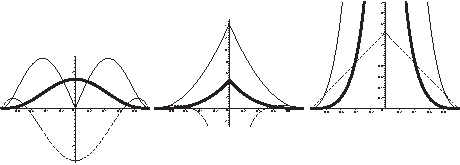
\includegraphics[width=\textwidth]{figures/smoothing-kernels.pdf}
  \caption[Πυρήνες εξομάλυνσης] {Οι τρεις πυρήνες εξομάλυνσης $W_{\text{\eng{poly6}}}$
    $W_{\text{\eng{spiky}}}$
    και $W_{\text{\eng{viscosity}}}$
    (από δεξιά προς τα αριστερά). Με τονισμένη γραμμή απεικονίζεται ο πυρήνας, με λεπτή η
    βάθμωσή του (στην κατεύθυνση προς την αρχή των αξόνων) και με διακεκομένη η λαπλασιανή
    του, για ακτίνα εξομάλυνσης $h=1$.
    (από \eng{M{\"u}ller et al, 2003}) \cite{muller2003particle}}
  \label{fig:smoothing-kernels}
\end{figure}

\paragraph{} Στο σχήμα \ref{fig:smoothing-kernels} φαίνονται οι τρεις πυρήνες
$W_{\text{\eng{poly6}}}$
$W_{\text{\eng{spiky}}}$
και $W_{\text{\eng{viscosity}}}$
που χρησιμοποιούνται πρακτικά για τον υπολογισμό της πυκνότητας, της βάθμωσης της πίεσης
και της λαπλασιανής του πεδίου ταχύτητας αντίστοιχα. Είναι σημαντικό για την ευστάθεια της
προσομοίωσης, αλλά και λογικό από φυσικής εποπτείας οι πυρήνες και οι παράγωγοι τους να
τείνουν στο μηδέν στα όρια της ακτίνας εξομάλυνσης. Για τον υπολογισμό της πυκνότητας
χρησιμοποιείται ο πυρήνας
\begin{equation}
  \label{eq:poly6}
  W_{\text{\eng{poly6}}}(r, h) = \frac{315}{64 \pi h^9}
  \begin{cases}
    (h^2 - r^2)^3 & 0 \leq r \leq h\\
    0 & \text{διαφορετικά}
  \end{cases}
\end{equation}
ο οποίος είναι τυπικός κωδωνοειδής πληρώντας τα χαρακτηριστικά που αναφέρθηκαν
προηγουμένως. Παρ' όλ' αυτά δε χρησιμοποιείται για την προσέγγιση της βάθμωσης της πίεσης,
καθότι η μηδενική παράγωγος στο κέντρο οδηγεί σε συσσωμάτωση (\eng{clustering}) των
σωματιδίων λόγω απουσίας απωστικών δυνάμεων μεταξύ τους. Για το λόγο αυτό, έχει προταθεί
\cite{desbrun1996smoothed} ο πυρήνας
\begin{equation}
  \label{eq:spiky}
  W_{\text{\eng{spiky}}}(r, h) = \frac{15}{\pi h^6}
  \begin{cases}
    (h - r)^3 & 0 \leq r \leq h\\
    0 & \text{διαφορετικά}
  \end{cases}
\end{equation}
\begin{equation}
  \label{eq:spiky-gradient}
  \nabla W_{\text{\eng{spiky}}}(r, h) = \frac{-45}{\pi h^6} (h-r)^2
\end{equation}
για τον υπολογισμό των δυνάμεων οφειλομένων στη βάθμωση της πίεσης. Ωστόσο οι δυνάμεις
ιξώδους είναι ανάλογες της λαπλασιανής του πυρήνα, με αποτέλεσμα οι παραπάνω πυρήνες να
είναι ακατάλληλοι για την προσέγγισή τους. Δεδομένου οτι οι δυνάμεις αυτές οφείλονται στην
εσωτερική τριβή του ρευστού, έχουν πάντα αποσβεστικά αποτελέσματα αμβλύνοντας τις τοπικές
διαφορές στην ταχύτητά του. Αντίθετα, οι λαπλασιανές των παραπάνω πυρήνων αλλάζουν αλλάζει
πρόσημο παίρνοντας αρνητικές τιμές. Έτσι υιοθετείται ο πυρήνας
\begin{equation}
  \label{eq:viscosity}
  W_{\text{\eng{viscosity}}}(r, h) = \frac{15}{2 \pi h^3}
  \begin{cases}
    - \frac{r^3}{2h^3} + \frac{r^2}{h^2} + \frac{h}{2r} - 1 & 0 \leq r \leq h\\
    0 & \text{διαφορετικά},
  \end{cases}\\
\end{equation}
\begin{equation}
  \label{eq:viscosity-laplacian}
  \nabla^2 W_{\text{\eng{viscosity}}}(r, h) = \frac{45}{\pi h^6} (h-r)
\end{equation}
ο οποίος έχει παντού θετική λαπλασιανή, της οποίας η γραμμικότητα συμβάλλει περαιτέρω στην
ευστάθεια της προσομοίωσης.

\subsubsection{Ολοκλήρωση και χρονικό βήμα}
\paragraph{} Εκτός της επιλογής του πυρήνα, καθοριστική για την ακρίβεια και ευστάθεια της
προσομοίωσης είναι η επιλογη του χρονικού βήματος και της μεθόδου ολοκλήρωσης στο
χρόνο. Το χρονικό βήμα υπολογίζεται συνήθως με βάση το κριτήριο \eng{CFL
  (Courant-Friedrichs-Lewy)} το οποίο στην απλούστερη μορφή του δίνεται από τη σχέση
\begin{equation}
  \label{eq:cfl}
  \delta t_{\text{\eng{CFL}}} = C \frac {\delta x}{v},
\end{equation}
όπου $C$
ο αδιάστατος αριθμός \eng{Courant} (συνήθως $0 < C \leq 1$),
$\delta x$
είναι κάποιο χαρακτηριστικό μήκος και $v$
μια σχετική με αυτό χαρακτηριστική ταχύτητα. Στην περίπτωση της \eng{SPH} μπορεί να
χρησιμοποιηθεί η ακτίνα εξομάλυνσης $h$
ή η ακτίνα των σωματιδίων σαν $\delta x$,
ενώ για την $v$
είτε η ταχύτητα του ήχου στο ρευστο, είτε η ταχύτητα των σωματιδίων για τη μέγιστη ανεκτή
μεταβολή πυκνότητας κατά τη διάρκεια ενός χρονικού βήματος, είτε η μέγιστη ταχύτητα των
σωματιδίων (αν μπορεί αυτή εκ των προτέρων να εκτιμηθεί με αξιοπιστία και δεν οδηγεί σε μη
αποδεκτές μεταβολές πυκνότητας). Μεταβλητό χρονικό βήμα μπορεί να χρησιμοποιηθεί υπό
προϋποθέσεις εξαρτώμενες και από την μέθοδο ολοκλήρωσης, με την προσαρμογή να λαμβάνει
χώρα σε κάθε βήμα της προσομοίωση με βάση το κριτήριο \eng{CFL} \cite{gomez2010state}.

\paragraph{} Για την αριθμητική ολοκλήρωση στο χρόνο χρησιμοποιούνται πολλές μέθοδοι,
μεταξύ των οποίων η \eng{predictor-corrector} και η \eng{Runge-Kutta-Fehlberg}. Ίσως η
ευρύτερα διαδεδομένη είναι η οικογένεια των \eng{St{\"o}rmer-Verlet} και \eng{Leapfrog},
οι οποίες είναι μέθοδοι δεύτερης τάξης με χαμηλές υπολογιστικές απαιτήσεις και καλή
αριθμητική ευστάθεια. Η μέθοδος \eng{Leapfrog} οφείλει το όνομά της στον αλληλοδιάδοχο
υπολογισμό της θέσης και της ταχύτας ανα μισό χρονικό βήμα
\begin{align}
  \begin{split}
    \label{eq:leapfrog}
    \vec{r}_{i+1} &= \vec{r}_i + \vec{v}_{i-1/2} \delta t \\
    \vec{v}_{i+1/2} &= \vec{v}_{i-1/2} + \vec{a}_i \delta t
  \end{split}
\end{align}
ή ισοδύναμα, σε ακέραια χρονικά βήματα
\begin{align}
  \begin{split}
    \label{eq:leapfrog}
    \vec{r}_{i+1} &= \vec{r}_i + \left( \vec{v}_i + \vec{a}_i \frac{\delta t}{2} \right) \delta t \\
    \vec{v}_{i+1} &= \vec{v}_i + \frac{\vec{a}_i + \vec{a}_{i+1}}{2} \delta t
  \end{split}
\end{align}
Λόγω της εξάρτησης των δυνάμεων (λ.χ. ιξώδους) και από την ταχύτητα στην \eng{SPH} μπορούν
να χρησιμοποιηθούν διάφορες τεχνικές εκτίμησης για τιμές στο μέλλον, όπως την επιτάχυνση
$\vec{a}_{i+1}$
\cite{rawiraswattana2012dynamics}.  Αυτές προσφέρουν παράλληλα τη δυνατότητα χρήσης
μεταβλητού χρονικού βήματος \cite{springel2001gadget}, η οποία δεν υπάρχει στην απλή
\eng{Leapfrog} μέθοδο, λόγω της εγγενούς συμμετρίας της \cite{skeel1993variable}.

%%% Local Variables:
%%% mode: latex
%%% TeX-master: "report"
%%% End:

\clearpage
\section{Υλοποίηση}

\paragraph{} Η προσομοίωση αποτελείται από δύο βασικά στοιχεία, την ακτογραμμή
(\eng{terrain}) και το ρευστό (\eng{fluid}). Το ρευστό είναι το δυναμικό στοιχείο, σε
αντίθεση με τη στατική ακτογραμμή. Στο πρόγραμμα προσομοίωσης, που στηρίζεται στη μηχανή
φυσικής \eng{Bullet}, δίνονται οι αρχικές συνθήκες του ρευστού (θέση και ταχύτητα) και
εισάγεται η ακτογραμμή με τη μορφή τρισδιάστατου τριγωνικού δικτύου επιφάνειας
(\eng{triangle surface mesh}). Στη συνέχεια εκτελείται η προσομοίωση και τα δεδομένα
εξάγονται σε αρχεία τύπου \eng{VTK} που μπορούν εισαχθούν σε ένα από τα πολλά προγράμματα
οπτικοποίησης που είναι διαθέσιμα ελεύθερα (λ.χ. \eng{ParaView}).

\subsection{\texorpdfstring{\eng{Bullet}}{}}
\label{ssec:bullet}
\paragraph{} Η \eng{Bullet} είναι μια μηχανή φυσικής που προσομοιώνει ανίχνευση και
χειρισμό συγκρούσεων καθώς και δυναμική εύκαμπτων και στερεών σωμάτων. Χρησιμοποιείται
ευρύτατα στην παραγωγή ηλεκτρονικών παιχνιδιών και οπτικών εφέ σε ταινίες, ενώ διατίθεται
ως ελεύθερο λογισμικό ανοιχτού πηγαίου κώδικα, αναπτυσσόμενη συνεχώς και υποστηριζόμενη
από μεγάλη και ενεργή κοινότητα χρηστών.

\paragraph{} Η \eng{Bullet} είναι σχεδιασμένη βάσει αντικειμενοστραφούς αρχιτεκτονικής,
καθώς οτιδήποτε, ακόμη και ο κόσμος της εξομοίωσης με τις όποιες ιδιότητές του
αναπαρίσταται με αντικείμενα, τα οποία δημιουργούνται, τροποποιούνται και καταστρέφονται
βάσει των αντίστοιχων μεθόδων της κλάσης τους. Ο κόσμος της προσομοίωσης, που ανήκει στην
κλάση \ttt{btDiscreteDynamicsWorld} δημιουργείται με βάση τέσσερα ορίσματα, εκ των οποίων
δύο (\ttt{btCollisionConfiguration} και \ttt{btDispatcher}) σχετίζονται με τους
αλγορίθμους χειρισμού συγκρούσεων και αφήνονται στις προεπιλεγμένες τους κλάσεις. Το τρίτο
όρισμα (\ttt{btBroadphaseInterface}) αφορά την οργάνωση των σωμάτων της προσομοίωσης στη
μνήμη με σκοπό τον εκ των προτέρων αποκλεισμό συγκρούσεων μεταξύ τους για την ελάφρυνση
του υπολογιστικού φόρτου. Στην παρούσα εργασία επιλέγεται η κλάση \ttt{btDbvtBroadphase} η
οποία ταξινομεί δυναμικά τα σώματα της προσομοίωσης σε δομή δένδρου με βάση τα
προσανατολισμένα με τους άξονες συντεταγμένων περιβάλλοντα κουτιά τους (\eng{AABBs}). Το
τελευταίο όρισμα (\ttt{btConstraintSolver}) καθορίζει τον τρόπο χειρισμού των γεωμετρικών
περιορισμών κατά την προσομοίωση. Εδώ επιλέγεται η χρήση του \eng{SIS} (\eng{Sequential
  Impulse Solver}) για την επίλυση πολλαπλών μηχανικών περιορισμών
\cite{catto2005iterative}. Τα σώματα της προσομοίωσης αρχικοποιούνται όπως περιγράφεται
στις παραγράφους παρακάτω και προστίθενται στον κόσμο της προσομοίωσης με τη μέθοδο
\ttt{addRigidBody}.

\paragraph{} Η προσομοίωση του κόσμου διεξάγεται σε διακριτά χρονικά βήματα μέσω της
μεθόδου \ttt{stepSimulation}, η οποία δέχεται τρία ορίσματα, έστω \ttt{T}, \ttt{k} και
\ttt{t} αντίστοιχα. Το πρώτο από αυτά καθορίζει το χρονικό διάστημα που θα προσομοιωθεί
συνολικά μέχρι το επόμενο στιγμιότυπο της προσομοίωσης (για συλλογή δεδομένων), το δεύτερο
το μέγιστο αριθμό εσωτερικών βημάτων εντός αυτού και το τρίτο τη χρονική διάρκεια του
εσωτερικού (αδιαίρετου) βήματος της προσομοίωσης (όπως είναι προφανές, θα πρέπει να ισχύει
\ttt{T$\geq$k*t}).
Η \eng{Bullet} παρέχει τη δυνατότητα ορισμού μιας \eng{callback} συνάρτησης, η οποία
καλείται μετά από κάθε εσωτερικό βήμα της προσομοίωσης και όπως θα αναλυθεί παρακάτω,
εκτελεί τον κώδικα που υλοποιεί τη μηχανή \eng{SPH} για την προσθήκη των δυνάμεων ρευστού
στα σωματίδια.

\subsection{Ακτογραμμή}
\paragraph{} Η ακτογραμμή αναπαρίσταται στο πρόγραμμα σαν ένα στατικό δίκτυο τριγώνων με
ιεραρχικούς περιβάλλοντες όγκους (\ttt{btBvhTriangleMesh}) της \eng{Bullet}. Τα δεδομένα
του τρισδιάστατου μοντέλου εισάγονται από ένα αρχείο τύπου \eng{obj} στο τριγωνικό δίκτυο
αφού κανονικοποιηθούν σε κλίμακα βάσει ενός παράγοντα κλιμάκωσης (\eng{scaling factor})
και θέση μετακινούμενα στο χώρο προς την αρχή των αξόνων (\eng{docking}). Γύρω από την
ακτογραμμή δημιουργείται και το όριό της (\eng{terrain boundary}) το οποίο ταυτίζεται με
το προσανατολισμένο στους άξονες περιβάλλον κουτί της (\eng{AABB}). Η κανονικοποιημένη
ακτογραμμή και το όριό της εξάγονται σε ένα αρχείο τύπου \eng{VTK}, το οποίο
χρησιμοποιείται για την οπτικοποίηση των δεδομένων. Σε κάθε εσωτερικό βήμα της
προσομοίωσης συλλέγονται οι ώσεις που ασκεί το ρευστό στην ακτογραμμή σε ειδικό διάνυσμα,
το οποίο χρησιμοποιείται για να εξαχθούν οι σχετικές πληροφορίες σε κάθε στιγμιότυπο.

\subsection{Ρευστό}
\subsubsection{Αρχικοποίηση}
\label{sssec:fluid-init}
\paragraph{} Σύμφωνα με τη μέθοδο \eng{SPH} όπως περιγράφηκε έως τώρα, το ρευστό
διακριτοποιείται σε σωματίδια τα οποία χρησιμοποιούνται σαν σημεία παρεμβολής σε
σταθμισμένα αθροίσματα για την εκτίμηση των ιδιοτήτων του ρευστού στο χώρο. Λόγω των
σημαντικών αποκλίσεων που μπορούν να προκύψουν εξαιτίας της έλλειψης γειτονικών
σωματιδίων, η μέθοδος ενδείκνυται κυρίως για την προσομοίωση συμπιεστών ρευστών (αερίων),
των οποίων η πυκνότητα δεν είναι σταθερή. Σε ασυμπίεστα ρευστά (υγρά) αντίθετα, όπου τα
όρια είναι σαφή, καθίσταται προβληματικός ο υπολογισμός ποσοτητων κοντά σε αυτά λόγω
μικρού αριθμού και ανομοιογενώς κατανεμημένων στο χώρο γειτονικών σωματιδίων. Για το λόγο
αυτό στην παρούσα προσομοίωση υιοθετήθηκε μια διαφορετική προσέγγιση, όπου τα σωματίδια
διαθέτουν υλική υπόσταση στερεών σφαιρών, η οποία μέσω επίλυσης γεωμετρικών περιορισμών σε
κάθε βήμα της προσομοίωσης (\eng{Position-Based Dynamics -- PBD} \cite{Muller2007109})
εξασφαλίζει την ασυμπιεστότητα του ρευστού \cite{macklin2013position}. Οι γεωμετρικοί
περιορισμοί επιλύονται από την \eng{Bullet}, αποκλείοντας τη δημιουργία εκφυλισμένων
περιπτώσεων όσον αφορά τις θέσεις των σωματιδίων, καθώς αυτά εμποδίζονται από το να
πλησιάσουν περισσότερο από την απόσταση που υπαγορεύει η ονομαστική πυκνότητα του
ρευστού. Επιπλέον, με τη μέθοδο αυτή διευκολύνεται ο χειρισμός των οριακών συνθηκών, χωρίς
να απαιτούνται επιπρόσθετες τεχνικές για την αναπλήρωση γειτονικών σωματιδίων. Για την
αρχικοποίηση του ρευστού δίνεται η θέση του στο χώρο, η αρχική ταχύτητα και το επιθυμητό
πλήθος των σωματιδίων στα οποία πρόκειται να διακριτοποιηθεί.

\paragraph{} Για την αρχικοποίηση του ρευστού δίνεται η θέση του στο χώρο, η αρχική
ταχύτητα και το επιθυμητό πλήθος σωματιδίων στα οποία πρόκειται να διακριτοποιηθεί. Τα
σωματίδια προγραμματιστικά είναι δομές \ttt{particle} που εμπλουτίζουν αντικείμενα στερεών
σωμάτων \ttt{btRigidBody} της \eng{Bullet} με πληροφορίες σχετιζόμενες με το ρευστό, όπως
πυκνότητα και πίεση. Η μάζα του ρευστού ισοκατανέμεται στα σωματίδια, τα οποία όντας
σφαιρικού σχήματος τοποθετούνται σε τρισδιάστατο εξαγωνικό πλέγμα \eng{HCP (Hexagonal
  Close-Packed)}, το οποίο επιτυγχάνει τη συνεκτικότερη δυνατή διευθέτηση ίσομεγεθών
σφαιρών με κλάσμα κάλυψης χώρου ίσο με $\pi/(3\sqrt{2})$.
Η ακτίνα των σωματιδίων υπολογίζεται από το κλάσμα αυτό και τον όγκο του ρευστού, ενώ η
ακτίνα εξομάλυνσης \ttt{h} τέτοια ώστε κάθε σωματίδιο να διαθέτει περίπου 50 γειτονικά
σωματίδια με τα οποία αλληλεπιδρά, αριθμός που προκύπτει εμπειρικά σύμφωνα με τη
βιβλιογραφία.

\paragraph{} Μετά την αρχικοποίηση εξάγονται παράμετροι της προσομοίωσης σχετικά με το
ρευστό:
\begin{description}
\item[Χρονικό βήμα] Το χρονικό βήμα καθορίζεται όπως έχει ήδη αναφερθεί από το κριτήριο
  ευστάθειας \eng{CFL}, με το χαρακτηριστικό μήκος να αποτελεί η ακτίνα των σωματιδίων και
  χαρακτηριστική ταχύτητα τη μέγιστη ταχύτητα των σωματιδίων με βάση την αρχική μηχανική
  ενέργεια του ρευστού.
\item[Πλήθος γειτόνων] Στην αρχική κατάσταση όπου τα σωματίδια είναι διευθετημένα στο
  πλέγμα \eng{HCP}, γίνεται ανίχνευση γειτόνων ώστε να μετρηθεί ο πραγματικός μέγιστος
  αριθμός γειτόνων ένός σωματιδίου (ο οποίος δεν είναι σχεδόν ποτέ ακριβώς 50 λόγω
  διακριτοποίησης).
\item[Καταστατική εξίσωση] Καθώς το πρόβλημα της ασυμπιεστότητας λύνεται άμεσα μέσω της
  επίλυσης γεωμετρικών περιορισμών μεταξύ των σωματιδίων, ως καταστατική εξίσωση
  χρησιμοποιείται η γραμμική των ιδανικών αερίων (σχέση \ref{eq:ideal-state}). Αυτή
  επιτρέπει μεγαλύτερο χρονικό βήμα και ανοχή όσον αφορά την ευστάθεια στις διακυμάνσεις
  της υπολογιζόμενης πυκνότητας. Σε περίπτωση υπολογισμού πολύ χαμηλής πυκνότητας
  μικρότερης από κάποιο κατώφλι (λ.χ. 0.9 της ονομαστικής) αυτή συμβατικά αντικαθίσταται
  από την ονομαστική, θεωρώντας οτι δεν υπάρχουν αρκετα γειτονικά σωματίδια για αξιόπιστη
  εκτίμηση.
\item[Συντελεστής πυκνότητας] Λόγω της εξάρτησης των πυρήνων εξομάλυνσης από την ακτίνα
  εξομάλυνσης, αλλά και της μάζας των σωματιδίων από τη διακριτοποίηση, το σταθμισμένο
  άθροισμα της εκτίμησης της πυκνότητας δεν ισούται με την πραγματική πυκνότητα του
  ρευστού, αλλά σχετίζεται αναλογικά με έναν συντελεστή, ο οποίος εξάγεται κατά το στάδιο
  αυτό. Ο συντελεστής αυτός χρησιμοποιείται για την αναλογική αντιστοίχιση της αδιάστατης
  πυκνότητας με την πραγματική και υπολογίζεται με βάση τη μέγιστη πυκνότητα των
  σωματιδίων κατά την ανίχνευση γειτόνων στην αρχική κατάσταση όπως αναφέρεται παραπάνω.
\end{description}

\subsubsection{Αναπαράσταση}
\label{sssec:lp-grid-representation}
\paragraph{} Στις προσομοιώσεις \eng{SPH} χρησιμοποιούνται διάφορες δομές δεδομένων με
σκοπό τη βελτιστοποίηση της πρόσβασης και ενημέρωσης σε γειτονικά σωματίδια. Σε αυτές
περιλαμβάνονται οι συνδεδεμένες λίστες \cite{monaghan1985refined, shao2003787}, δομές
δένδρων όπως το \eng{octree} \cite{losasso2004simulating}, απλά \eng{grid}
\cite{wang2012real}, καθώς και εξειδικευμένες δομές για \eng{GPUs}, όπως \eng{kd}-δένδρα
\cite{zhou2008real} και \eng{z-indexing} \cite{goswami2010interactive}. Για την καλύτερη
απόδοση της παρούσας προσομοίωσης αναπτύχθηκε εξειδικευμένη δομή δεδομένων, στο εξής
\eng{LP grid}. Ο χώρος της προσομοίωσης διαιρείται σε ένα κυβικό πλέγμα προσανατολισμένο
με το τρισορθογώνιο σύστημα συντεταγμένων, με το βήμα του πλέγματος (μήκος πλευράς των
κύβων) να ισούται με την ακτίνα εξομάλυνσης της προσομοίωσης. Με τον τρόπο αυτό όλοι οι
γείτονες ενός σωματιδίου βρίσκονται στα 26 κελιά που περιβάλλουν το κελι στο οποίο
ανήκει. Η διάταξη των κελιών στη μνήμη έχει στόχο την διατήρηση της τοπικότητας
(\eng{locality preserving}, εξ ου και η ονομασία), ώστε κελιά που βρίσκονται κοντά στον
τρισδιάστατο χώρο να βρίσκονται κοντά και στη μνήμη (η οποία είναι μονοδιάστατη και
γραμμική). Έτσι, με την αντιγραφή ενός τμήματος κυρίας μνήμης (\eng{RAM}) στην κρυφή μνήμη
(\eng{cache}) αυξάνεται η πιθανότητα τα δεδομένα γειτονικών σωματιδίων να μεταφέρονται
συντονισμένα στην κρυφή μνήμη, με αποτέλεσμα την αύξηση του λόγου \eng{hit}/\eng{miss} και
συνακόλουθα της ταχύτητας του προγράμματος.

\paragraph{Οργάνωση} Στη δομή \ttt{lp\_grid} αποθηκεύονται διάφορες παράμετροι της
προσομοίωσης όπως η αρχή του (\ttt{origin}), το βήμα του (\ttt{step} που ισούται με την
ακτίνα εξομάλυνσης \ttt{smoothing\_radius}), το πλήθος των κελιών κατά μήκος κάθε άξονα
(\ttt{x}, \ttt{y}, \ttt{z}), όπως και το πλήθος κελιών και σωματιδίων (\ttt{cell\_count},
\ttt{particle\_count}). Επίσης, όπως φαίνεται και στο σχήμα \ref{fig:lp-grid}, η δομή
περιλαμβάνει τρία διανύσματα δεικτών:
\begin{description}
\item[\ttt{MAP}] Στο διάνυσμα αυτό αποθηκεύονται δείκτες προς θέσεις εντός του
  \ttt{anchors}. Σκοπός του \ttt{map} είναι η διευθυνσιοδότηση σύμφωνα με τη βέλτιστη για
  τη διατήρηση της τοπικότητας διάταξή των κελιών (αντιστοίχιση τρισδιάστατου χώρου σε
  μονοδιάστατο). Διαθέτει \ttt{cell\_count+1} θέσεις, με το επιπλέον στοιχείο να
  αντιστοιχεί σε ένα εικονικό κελί που περιέχει σωματίδια εκτός ορίων του πλέγματος.
\item[\ttt{ANCHORS}] Κάθε δείκτης του διανύσματος αυτού σηματοδοτεί την αρχή του εκάστοτε
  κελιού (το πρώτο σωματίδιο) στο διάνυσμα \ttt{particles}. Τα κελιά αντιπροσωπεύονται
  διατεταγμένα προς διατήρηση τοπικότητας στο \ttt{anchors} και τα σωματίδια κάθε κελιού
  αποθηκεύονται σε διαδοχικές θέσεις του \ttt{particles}. Συνεπώς για τα στοιχεία του
  διανύσματος αυτού ισχύει \ttt{a[i-1]} $\leq$
  \ttt{a[i]} (στην περίπτωση που \ttt{a[i-1]} = \ttt{a[i]}, το κελί που αντιστοιχεί στο
  \ttt{a[i-1]} δεν περιέχει κανένα σωματίδιο). Το διάνυσμα διαθέτει και αυτό
  \ttt{cell\_count+1} θέσεις.
\item[\ttt{PARTICLES}] Το διάνυσμα αυτό διαθέτει \ttt{particle\_count+1} θέσεις και
  περιέχει τα σωματίδια της προσομοίωσης, ενώ κάθε πραγματικό κελί \ttt{i} στην
  προσομοίωση αντιπροσωπεύεται από το ζεύγος δεικτών \ttt{a[i]}, \ttt{a[i+1]}. Η επιπλέον
  θέση στο τέλος του διανύσματος χρησιμοποιείται για έγκυρο δείκτη τέλους του τελευταίου
  (εικονικού) κελιού (τα σωματίδια του οποίου αποθηκεύονται στις τελευταίες θέσεις του
  \ttt{particles}), καθώς και για έγκυρη αρχικοποίηση (κατά τη διάρκεια της οποίας, όπως
  θα φανεί παρακάτω, υπάρχει δείκτης προς τη θέση αυτή).
\end{description}
\begin{figure}[h]
  \centering
  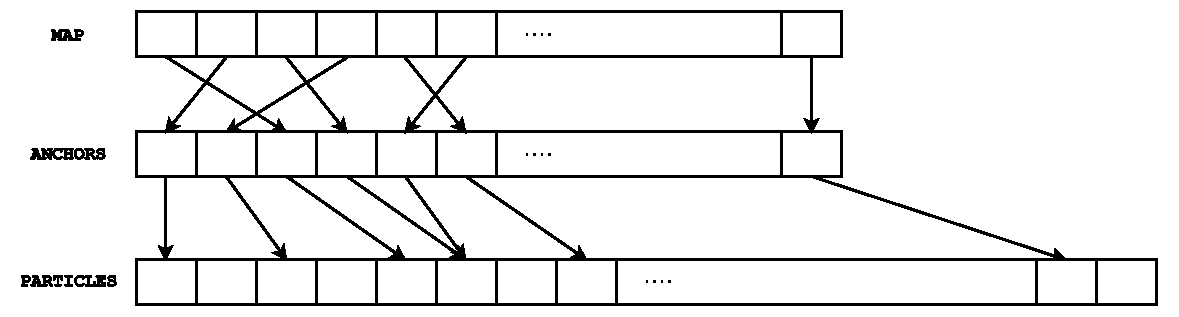
\includegraphics[width=\textwidth]{figures/lp-grid.pdf}
  \caption[Διανύσματα οργάνωσης του \ttt{lp\_grid}] {Τα τρία διανύσματα διευθυνσιοδότησης
    και αποθήκευσης του \ttt{lp\_grid}, μέσω των οποίων επιτυγχάνεται γρήγορη πρόσβαση και
    αποτελεσματική για τη διατήρηση της τοπικότητας διάταξη των σωματιδίων στη μνήμη.}
  \label{fig:lp-grid}
\end{figure}

\paragraph{} Η πρόσβαση στα κελιά του πλέγματος γίνεται με καθοδήγηση μέσω δεικτών
(\eng{pointer cascading}). Έστω οτι ζητούνται τα περιεχόμενα του κελιού στη διεύθυνση
\ttt{(i, j, k)} του πλέγματος. Η τρισδιάστατη διεύθυνση μετατρέπεται σε μονοδιάστατη (έναν
αριθμητικό δείκτη) μέσω μιας συνάρτησης \ttt{linearize}, η οποία αρκεί να υπολογίζει
διαφορετικό αποτέλεσμα για κάθε έγκυρη τρισδιάστατη διεύθυνση εισόδου και να έχει πεδίο
τιμών εντός του διαστήματος \ttt{[0, cell\_count]}, προκειμένου η έξοδος να αποτελεί
έγκυρη διεύθυνση για το διάνυσμα \ttt{map}. Τότε η αρχή του κελίου είναι ο δείκτης
\ttt{a[c] = *map[linearize(i, j, k)]} και το τέλος \ttt{a[c+1]}, με αποτέλεσμα τα
σωματίδια του κελιού να βρίσκονται με έναν απλό βρόχο επανάληψης ανάμεσα στους δύο
δείκτες, συμπεριλαμβανομένου του αρχικού, αλλά όχι του τελικού (δείκτης στο πρώτο
σωματίδιο του επόμενου κελιού).

\paragraph{Αρχικοποίηση} Η δημιουργία του \ttt{lp\_grid} γίνεται σε τέσσερα στάδια:
\begin{enumerate}
\item Καθορίζεται η αρχή του πλέγματος, το βήμα, το πλήθος κελιών και σωματιδίων του και
  δεσμεύεται βάσει αυτών χώρος στη μνήμη.

\item Τα κελιά του πλέγματος ταξινομούνται στο χώρο (\eng{spatial sort}) κατά μήκος μιας
  καμπύλης πλήρωσης χώρου (\eng{space-filling curve}, όπως η διάταξη \eng{Z} και η καμπύλη
  \eng{Hilbert}), με στόχο τη διατήρηση της τοπικότητας στην τελική γραμμική διάταξη κατά
  το μέγιστο δυνατό βαθμό. Στη συνέχεια αρχικοποιείται το διάνυσμα \ttt{map}, ώστε στη
  θέση \ttt{map[linearize(i, j, k)]} να υπάρχει δείκτης στην αντίστοιχη θέση του
  \ttt{anchors} σύμφωνα με τη χωρική ταξινόμηση των κελιών.

\item Κατασκευάζεται το διάνυσμα \ttt{cell\_pc} στις θέσεις του οποίου αποθηκεύεται το
  πλήθος των σωματιδίων σε κάθε κελί. Κατά τη διαδικασία αυτή χρησιμοποιείται η συνάρτηση
  \ttt{particle\_anchor}, η οποία παίρ\-νει ως όρισμα το \ttt{lp\_grid} και ένα σωματίδιο
  και επιστρέφει ένα δείκτη στον \ttt{anchor} του κελιού που περιέχει το σωματίδιο. Στη
  συνέχεια σύμφωνα με το \ttt{cell\_pc} αρχικοποιούνται οι δείκτες στο διάνυσμα
  \ttt{anchors}.

\item Τα σωματίδια αποθηκεύονται στο διάνυσμα \ttt{particles}, στη θέση που δείχνει ο
  \ttt{anchor} του κελιού που ανήκουν, ενώ μετά από κάθε προσθήκη ο \ttt{anchor} αυξάνεται
  κατά 1 (δείχνει στην επόμενη θέση του \ttt{particles}). Στο τέλος της διαδικασίας κάθε
  \ttt{anchor} δείχνει στην αρχή του επόμενου κελιού (και ο τελευταίος στην τελευταία
  επιπλέον θέση του \ttt{particles}). Ο πρώτος \ttt{anchor} επαναφέρεται στην αρχή του
  \ttt{particles} και κάθε επόμενος εκεί που δείχνει ο προηγούμενός του.
\end{enumerate}
Ακολουθεί ψευδοκώδικας για τη συνάρτηση \ttt{make\_lp\_grid} που δημιουργεί ένα
\ttt{lp\_grid}\footnote{Ονόματα μεταβλητών που λήγουν σε \ttt{p} υποδηλώνουν οτι η
  μεταβλητή αποτελεί δείκτη}: \selectlanguage{english}
\begin{verbatim}
lp_grid make_lp_grid(domain dom, fluid fl)
|   lp_grid lpg;
|   allocate_lp_grid (&lpg, dom, fl);
|   point cc[lpg.cell_count] = spatial_sort(collect_cell_centers(lpg));
|
|   // MAP initialization according to spatial sort.
|   for int i = 0 below lpg.cell_count:
|   |   lpg.map[linearize(cc[i].x, cc[i].y, cc[i].z)] = lpg.anchors + i;
|   lpg.map[lpg.cell_count] = lpg.anchors + lpg.cell_count;
|
|   // Store the particle count for each cell.
|   ptrdiff cell_pc[lpg.cell_count+1] = {0};
|   for particle p in fl.particles:
|   |   cell_pc[particle_anchor(lpg, p) - lpg.anchors]++;
|   for int anchor_offset = 0; int i = 0 upto lpg.cell_count:
|   |   lpg.anchors[i] = lpg.particles + anchor_offset;
|   |   anchor_offset += cell_pc[i];
|
|   // Populate particle array and reset anchors
|   for particle p in fl.particles:
|   |   anchor* ap = particle_anchor(lpg, p);
|   |   **ap = p;
|   |   (*ap)++;
|   for int i = lpg.cell_count above 0:
|   |   lpg.anchors[ai] = lpg.anchors[ai-1];
|   lpg.anchors[0] = lpg.particles;
|
|   return lpg;
\end{verbatim}
\selectlanguage{greek}

\paragraph{Ενημέρωση} Μετά από κάθε βήμα της προσομοίωσης τα σωματίδια έχοντας μετακινηθεί
ενδέχεται να βρίσκονται σε διαφορετικό κελί του πλέγματος, το οποίο πρέπει πλέον να
ενημερωθεί. Τα σωματίδια ελέγχονται με τη σειρά και σε περίπτωση σφάλματος, γίνεται
κυκλική μετακίνηση κατά μία θέση (\eng{shift}) δεξιά/αριστερά στο τμήμα του διανύσματος
\ttt{particles} μεταξύ της τρέχουσας και ορθής θέσης του σωματιδίου και αντίστοιχη
μετακίνηση ($\pm 1$) των \ttt{anchors} του τμήματος αυτού. Στη χειρότερη περίπτωση η
διαδικασία αυτή έχει απαγορευτική ασυμπτωτική συμπεριφορά ($Ο(n^2)$) σε συνήθεις όμως
περιπτώσεις απαιτεί πολύ λιγότερο χρόνο, διότι:
\begin{itemize}
\item Κατά κανόνα μικρό πλήθος σωματιδίων αλλάζουν κελί σε κάθε βήμα, δεδομένου οτι τα
  κελιά είναι αρκετά μεγάλα σε σχέση με το μέγεθος και την ταχύτητα των σωματιδίων.
  
\item Η διατήρηση της τοπικότητας εξασφαλίζει οτι τα κελιά άφιξης και προορισμού του
  σωματιδίου (τα οποία αναμένεται να είναι γειτονικά σε λογικό χρονικό βήμα) βρίσκονται
  κοντά στη γραμμική αναπαράσταση, με αποτέλεσμα η διαδικασία ενημέρωσης να αφορά μικρό
  τμήμα των διανυσμάτων \ttt{particles} και \ttt{anchors}.
\end{itemize}

\paragraph{} Στη συνέχεια παρατίθεται ψευδοκώδικας για τη συνάρτηση
\ttt{update\_lp\_grid}\footnote{Μεταβλητές των οποίων το όνομα ξεκινά με \ttt{i} αφορούν
  την τρέχουσα/αρχική θέση του σωματιδίου (\eng{initial}) πριν την ενημέρωση, ενώ με
  \ttt{t} την τελική/ορθή (\eng{terminal})}: \selectlanguage{english}
\begin{verbatim}
void update_lp_grid (lp_grid lpg)
|   anchor ta;
|   particle tmp_storage;
|   for anchor* iap = lpg.anchors below lpg.anchors + lpg.cell_count:
|   |   for anchor ia = *iap below *(iap + 1):
|   |   |   anchor* tap = particle_anchor(lpg, *ia);
|   |   |   if iap != tap:
|   |   |   |   tmp_storage = *ia;
|   |   |   |   if iap < tap:
|   |   |   |   |   ta = *tap - 1;
|   |   |   |   |   for anchor* ap = iap + 1 upto tap: (*ap)--;
|   |   |   |   |   for anchor a = ia below ta: *a = *(a + 1);
|   |   |   |   |   *ta = tmp_storage;
|   |   |   |   |   ia--;
|   |   |   |   else:
|   |   |   |   |   ta = *(tap + 1);
|   |   |   |   |   for anchor* ap = iap above tap: (*ap)++;
|   |   |   |   |   for anchor a = ia above ta: *a = *(a - 1);
|   |   |   |   |   *ta = tmp_storage;
|   return;
\end{verbatim}
\selectlanguage{greek}

\paragraph{} Όπως φαίνεται παραπάνω, στο βρόχο επανάληψης ελέγχεται κάθε σωματίδιο για το
αν βρίσκεται αποθηκευμένο στο τμήμα του \ttt{particles} που αντιστοιχεί στο κελί στο οποίο
βρίσκεται βάσει της θέσης του στο χώρο. Αν βρίσκεται αριστερότερα, μετακινείται στην πρώτη
θέση του ορθού κελιού αποθήκευσης μέσω αριστερής κυκλικής ολίσθησης ανάμεσα στις δύο
θέσεις, ενώ στην αντίθετη περίπτωση μετακινείται στην τελευταία του θέση μέσω δεξιάς
κυκλικής ολίσθησης μεταξύ αυτών των θέσεων. Στη συνέχεια ενημερώνονται κατάλληλα οι
\ttt{anchors} που δείχνουν στο τμήμα όπου λαμβάνει χώρα η ολίσθηση. Τέλος, στην περίπτωση
αριστερής ολίσθησης στην τρέχουσα θέση του βρόχου ελέγχου βρίσκεται μη ελεγμένο σωματίδιο
και για το λόγο αυτό η μεταβλητή ελέγχου του βρόχου \ttt{ia} μειώνεται κατά ένα (ο έλεγχος
γίνεται από τα αριστερά προς τα δεξιά στο διάνυσμα \ttt{particles}).

\subsubsection{Προσομοίωση}
\label{sssec:simulation}
\paragraph{} Για τον υπολογισμό των ιδιοτήτων του ρευστού είναι απαραίτητος ο υπολογισμός
πολλών σταθμισμένων αθροισμάτων που εξαρτώνται απο τις ιδιότητες αλλά και την απόσταση
μεταξύ σωματιδίων. Για να εξασφαλιστεί η διατήρηση της ορμής, οι αμοιβαίες συνεισφορές στα
αθροίσματα αυτά συμμετρικοποιούνται (\ref{sssec:vector-calc}), με αποτέλεσμα να λαμβάνουν
τη μορφή αλληλεπίδρασης. Συνεπώς ο υπολογιστικός φόρτος μειώνεται στο μισό εάν κάθε
αλληλεπίδραση ληφθεί υποψη μία φορά για κάθε ζεύγος σωματιδίων, εξετάζοντας μόνο τα μισά
κελιά γύρω από το τρεχον κελί κατά τη σάρωση του πλέγματος (αυτά που έχουν ελεγχθεί
νωρίτερα, προκειμένουν να αυξηθεί η πιθανότητα τα σωματίδιά τους να βρίσκονται ήδη στην
κρυφή μνήμη). H σάρωση του πλέγματος εκτελείται παράλληλα από πολλά νήματα
(\eng{threads}), μετά το διαχωρισμό του πλέγματος σε τμήματα (\eng{segments}) καταλλήλου
μεγέθους, το οποίο καθορίζεται κατά την αρχικοποίηση του \eng{LP grid}. Εμπειρικά
υιοθετήθηκε ως μέγεθος τμήματος σε κάθε διάσταση η τετραγωνική ρίζα του μήκους της, καθώς
επιτυγχάνει ικανοποιητικό συμβιβασμό μεταξύ κατανομής υπολογιστικού φόρτου (\eng{load
  distribution}) και επιπρόσθετου έργου (\eng{overhead}).

\paragraph{} Η προσομοίωση πραγματοποιείται σε σταθερό εσωτερικό χρονικό βήμα και ανά
συγκεκριμένο αριθμό βημάτων εξάγεται και ένα στιγμιότυπο (\eng{frame}), το οποίο περιέχει
πληροφορίες για τα σωματίδια, το ρευστό και την ακτογραμμή. Τα αρχεία \eng{VTK} που
αναπαριστούν το στιγμιότυπο ονομάζονται σύμφωνα με τον αύξοντα αριθμό αυτού, ώστε τελικά
να σχηματίζουν μια χρονοσειρά (\eng{file-} ή \eng{time-series}). Οι συγκρούσεις και οι
περιορισμοί ανάμεσα στα υλικά σώματα επιλύονται από την \eng{Bullet}, ενώ οι εσωτερικές
δυνάμεις του ρευστού υπολογίζονται μέσω κατάλληλα ορισμένης συνάρτησης που καλείται μετά
από κάθε εσωτερικό βήμα στον κύριο βρόχο της προσομοίωσης (\eng{tick callback}). Συνοπτικά
εντός αυτής εκτελούνται τα εξής βήματα:

\begin{enumerate}
\item Καταγραφή/αποθήκευση των ώσεων (\eng{impulses}) του ρευστού προς την ακτογραμμή.

\item Ενημέρωση του πλέγματος αποθήκευσης των σωματιδίων.

\item Καθαρισμός δεδομένων των σωματιδίων που πρόκειται να επανυπολογιστούν.

\item Ανιχνευση αλληλεπιδράσεων με σάρωση όλου του πλέγματος.

\item Υπολογισμός πυκνότητας στις θέσεις των σωματιδίων μέσω προοδευτικής άθροισης των
  αμοιβαίων συνεισφορών των αλληλεπιδρώντων ζευγών.

\item Υπολογισμός πίεσης στις ίδιες θέσεις μέσω της καταστατικής εξίσωσης του ρευστού,
  συναρτήσει της πυκνότητας.

\item Υπολογισμός και εφαρμογή των ώσεων που υπολογίζονται ως το γινόμενο των δυνάμεων
  πίεσης/ιξώδους και του χρονικού βήματος. Οι δυνάμεις είναι αντισυμμετρικές σε κάθε
  ζεύγος αλληλεπίδρασης, και οι μεν πίεσης είναι ανάλογες της διαφοράς πίεσης μεταξύ των
  δύο σημείων, οι δε ιξώδους της διαφοράς ταχυτήτων.
\end{enumerate}

\paragraph{} Για την ανακατασκευή της επιφάνειας του ρευστού υπολογίζεται σε διατεταγμένα
σημεία το χρωματικό πεδίο (\eng{color field}), ένα βαθμωτό πεδίο που ισοδυναμεί με την
αδιάστατη πυκνότητα του ρευστού σε κάθε σημείο του χώρου (δηλαδή υπό την παραδοχή οτι κάθε
σωματίδιο έχει μάζα ίση με 1). Τα κελιά του πλέγματος υποδιαιρούνται σε κυβικά υποκελιά,
στις γωνίες των οποίων υπολογίζονται οι τιμές του χρωματικού πεδίου, από τις οποίες στη
συνέχεια οπτικοποιείται η επιφάνεια του ρευστού ως ισοεπιφάνεια του πεδίου. Παρόμοια, για
τη συνολική απεικόνιση των ώσεων του ρευστού προς την ακτογραμμή, κατασκευάζεται το
αθροιστικό πεδίο ώσεων (\eng{impulse field}). Τα δείγματα του πεδίου αυτού υπολογίζονται
στα ίδια σημεία με το χρωματικό πεδίο προσθέτοντας το μέτρο κάθε καταγραφόμενης ώσης στο
κοντινότερο σημείο δειγματοληψίας μετά από κάθε βήμα της προσομοίωσης.

%%% Local Variables:
%%% mode: latex
%%% TeX-master: "report"
%%% End:

\clearpage
\section{Αξιολόγηση -- Αποτελέσματα}

\subsection{Προσομοιώσεις}

\paragraph{} Στην ενότητα αυτή παρουσιάζονται τα αποτελέσματα διαφόρων προσομοιώσεων. Τα
αποτελέσματα εξάγονται από το πρόγραμμα προσομοίωσης με τη μορφή αρχείων κειμένου
\eng{VTK}, τα οποία στη συνέχεια μπορούν να οπτικοποιηθούν και να διερευνηθούν διαδραστικά
μέσω διαφόρων ειδικών προγραμμάτων. Στην παρούσα εργασία, ως πρόγραμμα οπτικοποίησης
χρησιμοποιήθηκε το \eng{ParaView}, που αναπτύσσεται και διανέμεται ως ελεύθερο λογισμικό
από το \eng{Los Alamos National Laboratory}, το \eng{Sandia National Laboratory} και την
εταιρεία \eng{Kitware}. Το \eng{ParaView} τρέχει σε όλα τα ευρέως χρησιμοποιούμενα
λειτουργικά συστήματα (\eng{Unix/Linux, MS Windows, Mac OS X}), διαθέτει αρχιτεκτονική
\eng{client - server} για την οπτικοποίηση δεδομένων που βρίσκονται σε δίκτυο, υποστηρίζει
αρχιτεκτονικές κατανεμημένης επεξεργασίας ενώ δημιουργεί \eng{LOD} (\eng{Level of Detail})
οπτικοποιήσεις για την διατήρηση διαδραστικού αριθμού \eng{FPS} ακόμα και για μεγάλου
όγκου δεδομένα.

\begin{sidewaysfigure}
  \centering
  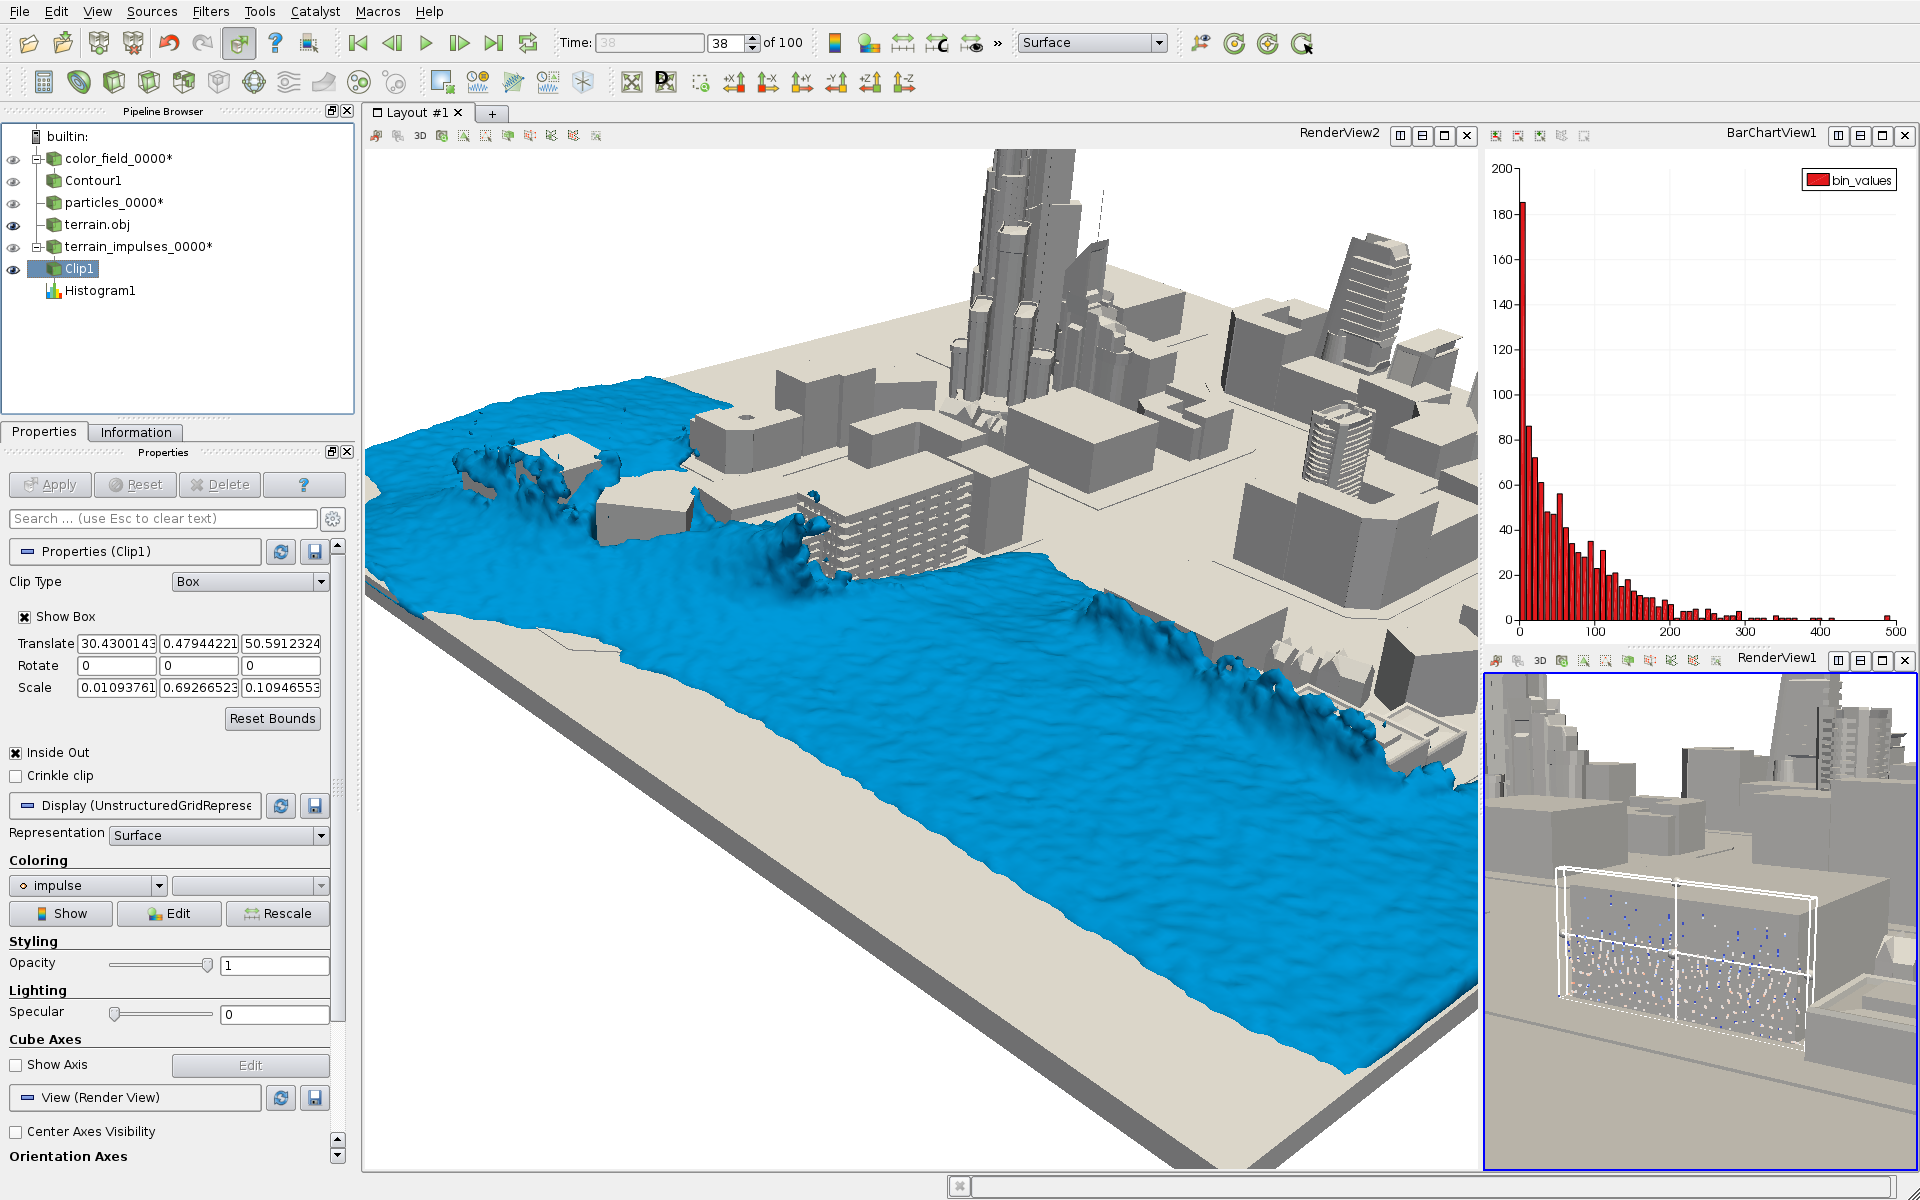
\includegraphics[width=\textwidth]{figures/paraview-interface.png}
  \caption[Οπτικοποίηση προσομοίωσης] {Οπτικοποίηση προσομοίωσης τσουνάμι \eng{85k}
    σωματιδίων στο \eng{ParaView}, στιγμιότυπο οθόνης. Αριστερά φαίνεται το ιεραρχικό
    δένδρο των δεδομένων που οπτικοποιούνται, στη μέση η ανακατασκευή της επιφάνειας του
    ρευστού σε συνδυασμό με το μοντέλο της ακτογραμμής, ενώ δεξιά οι ώσεις που ασκεί το
    ρευστό στο επιλεγμένο τμήμα του μοντέλου καθώς και γραφική απεικόνιση αυτών σε
    ιστόγραμμα.}
  \label{fig:paraview-interface}
\end{sidewaysfigure}

\paragraph{} Στην εικόνα \ref{fig:paraview-interface} φαίνεται σε στιγμιότυπο οθόνης το
περιβάλλον του \eng{ParaView} κατά την οπτικοποίηση μιας προσομοίωσης \eng{85k}
σωματιδίων. Στην αριστερή στήλη διακρίνεται το δένδρο με τις χρονοσειρές δεδομένων, στο
κορυφαίο επίπεδο του οποίου υπάρχουν το χρωματικό πεδίο (\eng{color\_field}), τα σωματίδια
της προσομοίωσης (\eng{particles}), οι ώσεις του ρευστού προς την ακτογραμμή
(\eng{terrain\_impulses}) και το μοντέλο της ακτογραμμής (\eng{terrain.obj}). Το ίδιο
σύνολο δεδομένων μπορεί να οπτικοποιηθεί ταυτόχρονα με πολλούς τρόπους, σε διάφορα
\eng{RenderViews}. Στο \eng{RenderView2} έχει επιλεγεί η απεικόνιση του μοντέλου της
ακτογραμμής σε γενική άποψη καθώς και της ισοεπιφάνειας του χρωματικού πεδίου, η οποία
δεδομένου ότι το χρωματικό πεδίο αντιπροσωπεύει την αδιάστατη πυκνότητα του ρευστού
αποτελεί μια αποδεκτή προσεγγιστική ανακατασκευή της επιφάνειάς του. Στο \eng{RenderView1}
έχει επιλεγεί η εστιασμένη απεικόνιση τμήματος της ακτογραμμής σε συνδυασμό με τις εντός
του κουτιού επιλογής (\eng{clip}) ώσεις προς αυτήν, οι οποίες είναι χρωματικά διαφορετικές
αναλόγως του μεγέθους τους και αναπαρίστανται σε ιστόγραμμα (\eng{BarChartView1}), όπου
είναι εύκολο να παρατηρηθεί η κατανομή της ορμής στα σωματίδια.

\begin{figure}[]
  \begin{subfigure}{.5\textwidth}
    \centering
    \includegraphics[width=\textwidth]{figures/press-0.png}
  \end{subfigure}
  \begin{subfigure}{.5\textwidth}
    \centering
    \includegraphics[width=\textwidth]{figures/press-1.png}
  \end{subfigure}
  \begin{subfigure}{.5\textwidth}
    \centering
    \includegraphics[width=\textwidth]{figures/press-2.png}
  \end{subfigure}
  \begin{subfigure}{.5\textwidth}
    \centering
    \includegraphics[width=\textwidth]{figures/press-3.png}
  \end{subfigure}
  \begin{subfigure}{.5\textwidth}
    \centering
    \includegraphics[width=\textwidth]{figures/press-4.png}
  \end{subfigure}
  \begin{subfigure}{.5\textwidth}
    \centering
    \includegraphics[width=\textwidth]{figures/press-5.png}
  \end{subfigure}
  \caption[Διάδοση δυνάμεων πίεσης]{Διαδοχικά στιγμιότυπα προσομοίωσης όπου αποτυπώνεται η
    διάδοση της ώσης του εδάφους στη υπερκείμενη στήλη νερού με τη μορφή δυνάμεων
    πίεσης. Τα σωματίδια της προσομοίωσης αναπαρίστανται με σημεία χρωματισμένα σύμφωνα με
    το μέτρο των δυνάμεων πίεσης που ασκούνται στο καθένα (θερμότητα χρώματος ανάλογη του
    μέτρου της δύναμης).}
  \label{fig:pressure-forces}
\end{figure}

\paragraph{} Όσον αφορά τις δυνάμεις που ασκούνται εντός του ρευστού, στις εικόνες
\ref{fig:pressure-forces} και \ref{fig:viscosity-forces} απεικονίζονται σε διαδοχικά
στιγμιότυπα τα σωματίδια της ίδιας προσομοίωσης, χρωματικά κωδικοποιημένα με βάση τις
δυνάμεις που ασκούνται σε αυτά λόγω πίεσης και ιξώδους αντίστοιχα. Το τσουνάμι
αναπαρίσταται σαν ένας όγκος νερού που εισβάλλει στην ακτογραμμή με μια σταθερή
ταχύτητα. Η προσέγγιση αυτή βρίσκεται αρκετά κοντά στην πραγματικότητα, δεδομένου οτι τα
τσουνάμι εκδηλώνονται ως μερικές επαναλαμβανόμενες, ορμητικές παλλίροιες της θάλασσας, με
μεγάλους όγκους νερού να ρέουν προς την ενδοχώρα. Στην εικόνα \ref{fig:pressure-forces}
παρατηρείται η διάδοση της ώσης του εδάφους στα αρχικά στάδια της προσομοίωσης μέσω
δυνάμεων πίεσης στη σχετικά άθικτη ακόμα υδάτινη στήλη (θερμότητα χρώματος ανάλογη του
μέτρου της δύναμης). Παρόμοια χρωματισμένες στην εικόνα \ref{fig:viscosity-forces}
διακρίνονται οι δυνάμεις ιξώδους, που οφείλονται στη διαφορά ταχύτητας μεταξύ γειτονικών
σωματιδίων και ως εκ τούτου είναι ισχυρές κατά την πρόσκρουση του ρευστού σε εμπόδια, όπου
τμήματά του αλλάζούν ταχύτητα σε σχέση με τα κοντινά τους. Στην εικόνα \ref{fig:samples}
τα σωματίδια κωδικοποιούνται χρωματικά σύμφωνα με το πλήθος γειτονικών σωματιδίων εντός
της ακτίνας εξομάλυνσης της προσομοίωσης. Όπως φαίνεται, λόγω της φύσης της προσομοίωσης
(ροή σε ανοιχτό χώρο με πολύπλοκα όρια) το ρευστό διαθέτει υψηλό λόγο επιφάνειας προς
όγκο, με αποτέλεσμα μεγάλο του μέρος να υποφέρει από υποδειγματοληψία. Για το λόγο αυτό
υιο\-θε\-τή\-θη\-καν (όπως αναλύθηκε και στην παράγραφο \ref{sssec:fluid-init})
γεωμετρικοί περιορισμοί μεταξύ των σωματιδίων για την αναπλήρωση της χαμένης πληροφορίας.

\begin{sidewaysfigure}[]
  \begin{subfigure}{.5\textwidth}
    \centering
    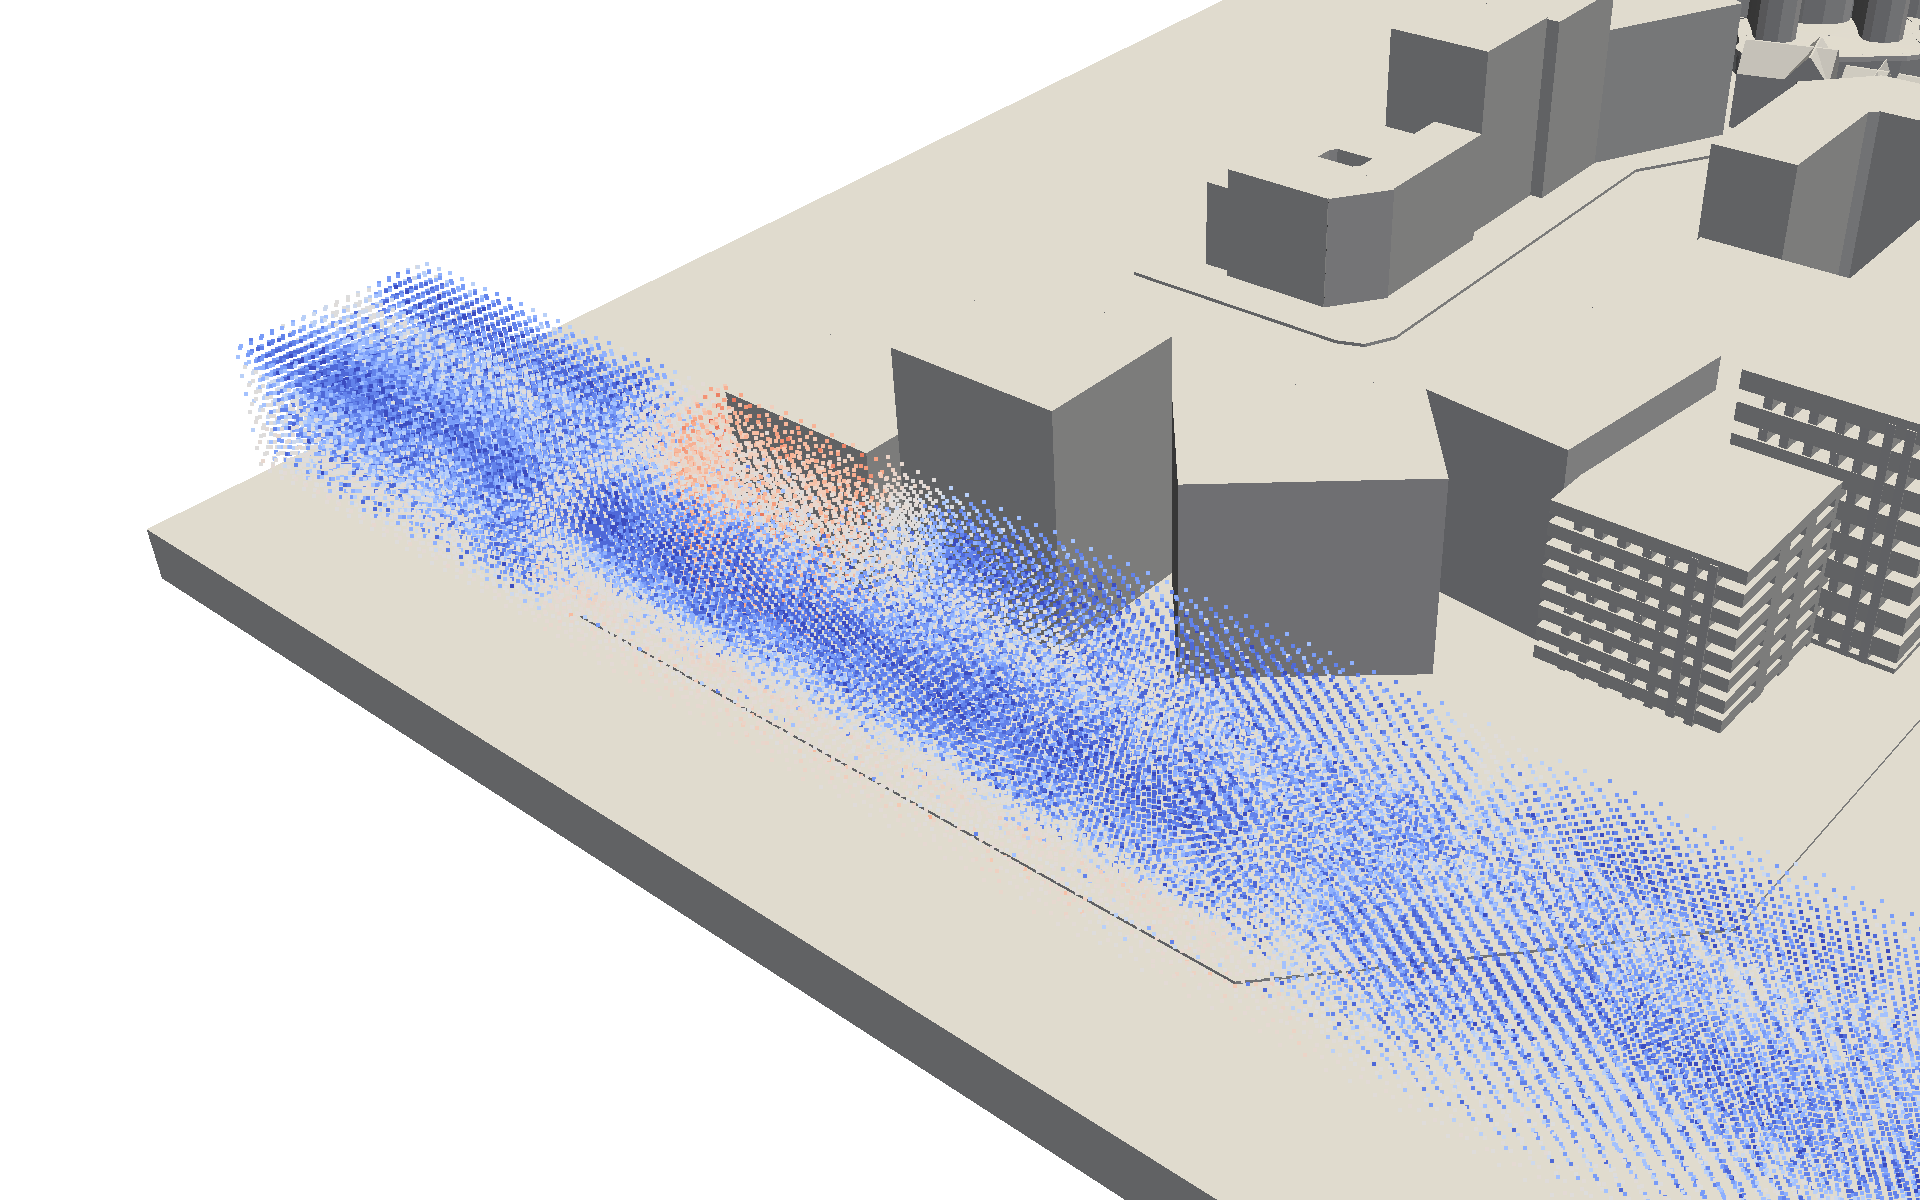
\includegraphics[width=\textwidth]{figures/visc-0.png}
  \end{subfigure}
  \begin{subfigure}{.5\textwidth}
    \centering
    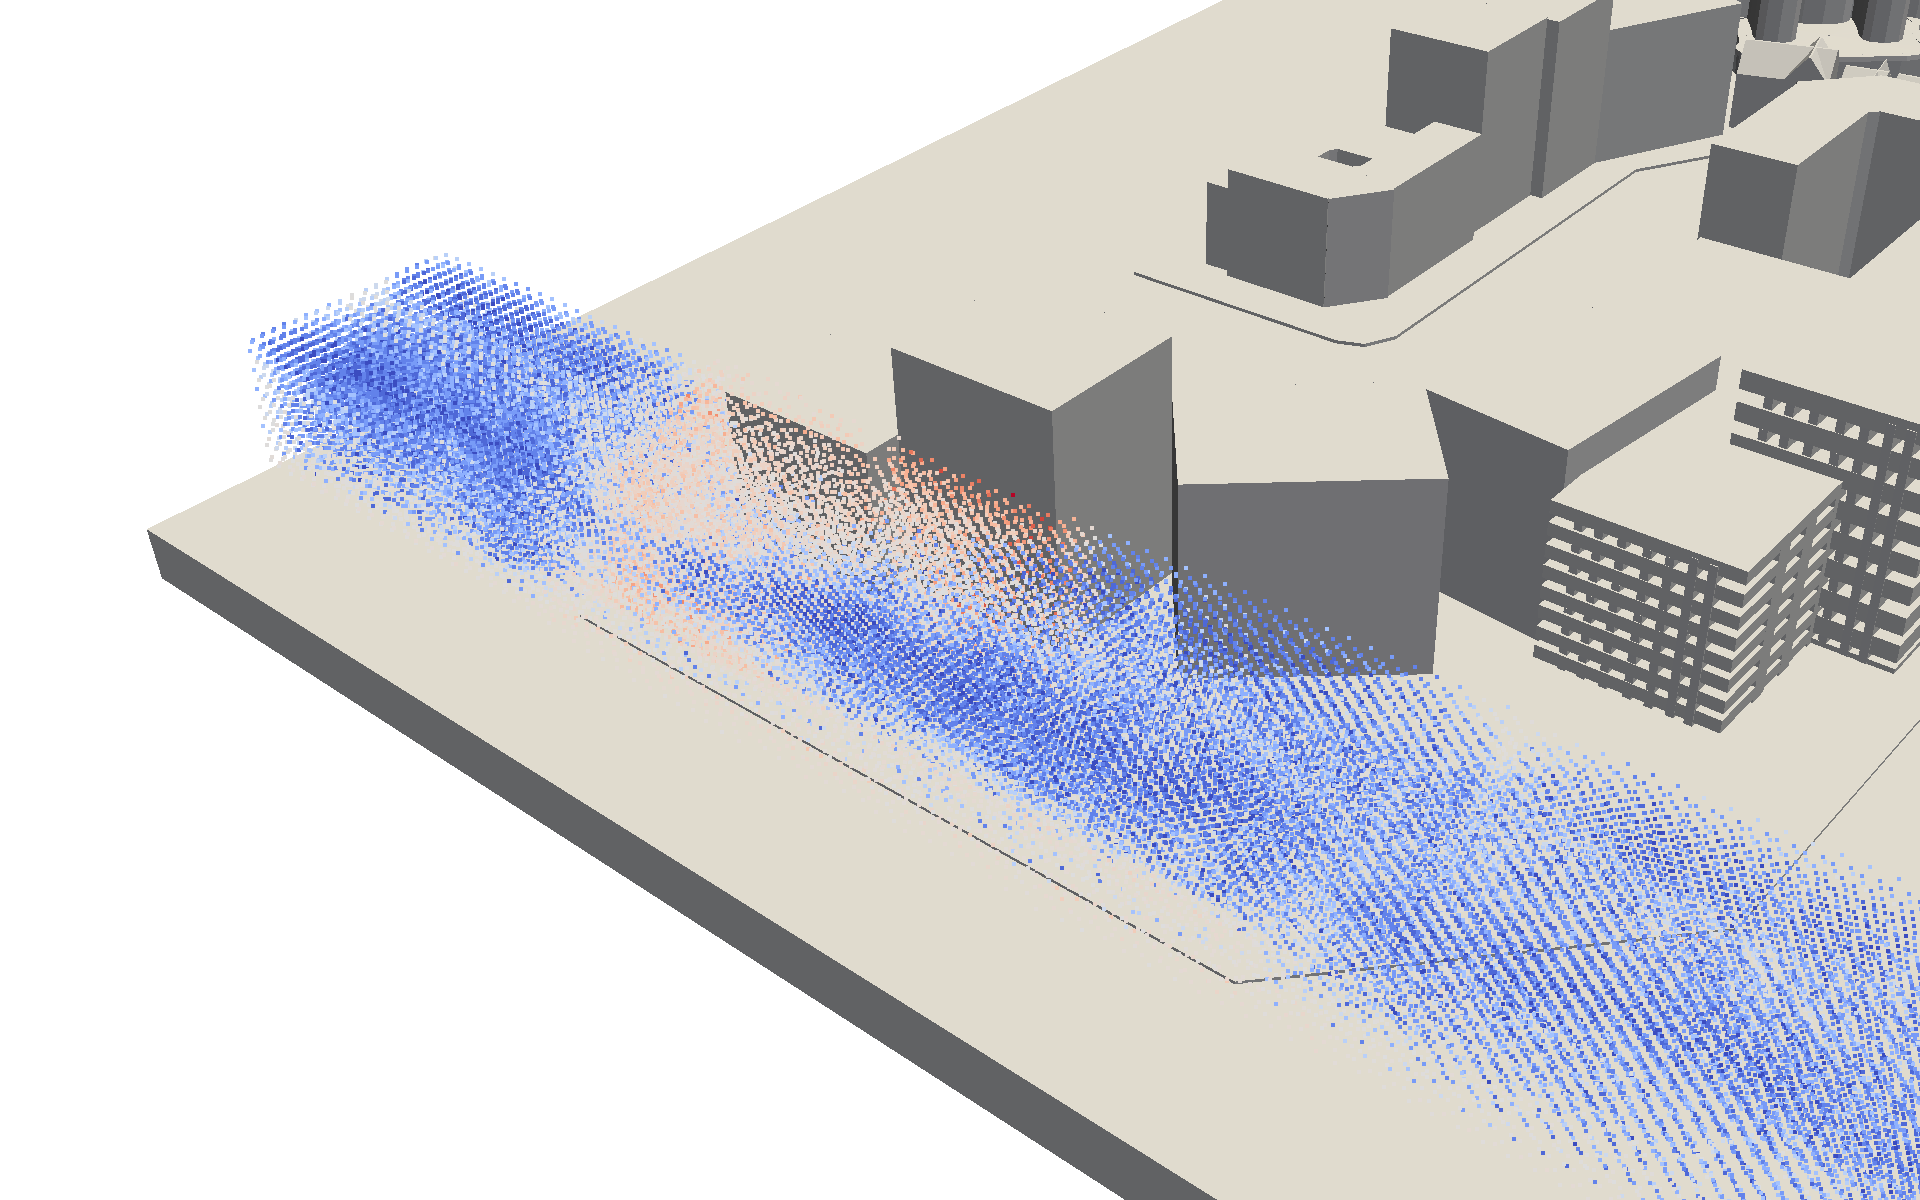
\includegraphics[width=\textwidth]{figures/visc-1.png}
  \end{subfigure}
  \begin{subfigure}{.5\textwidth}
    \centering
    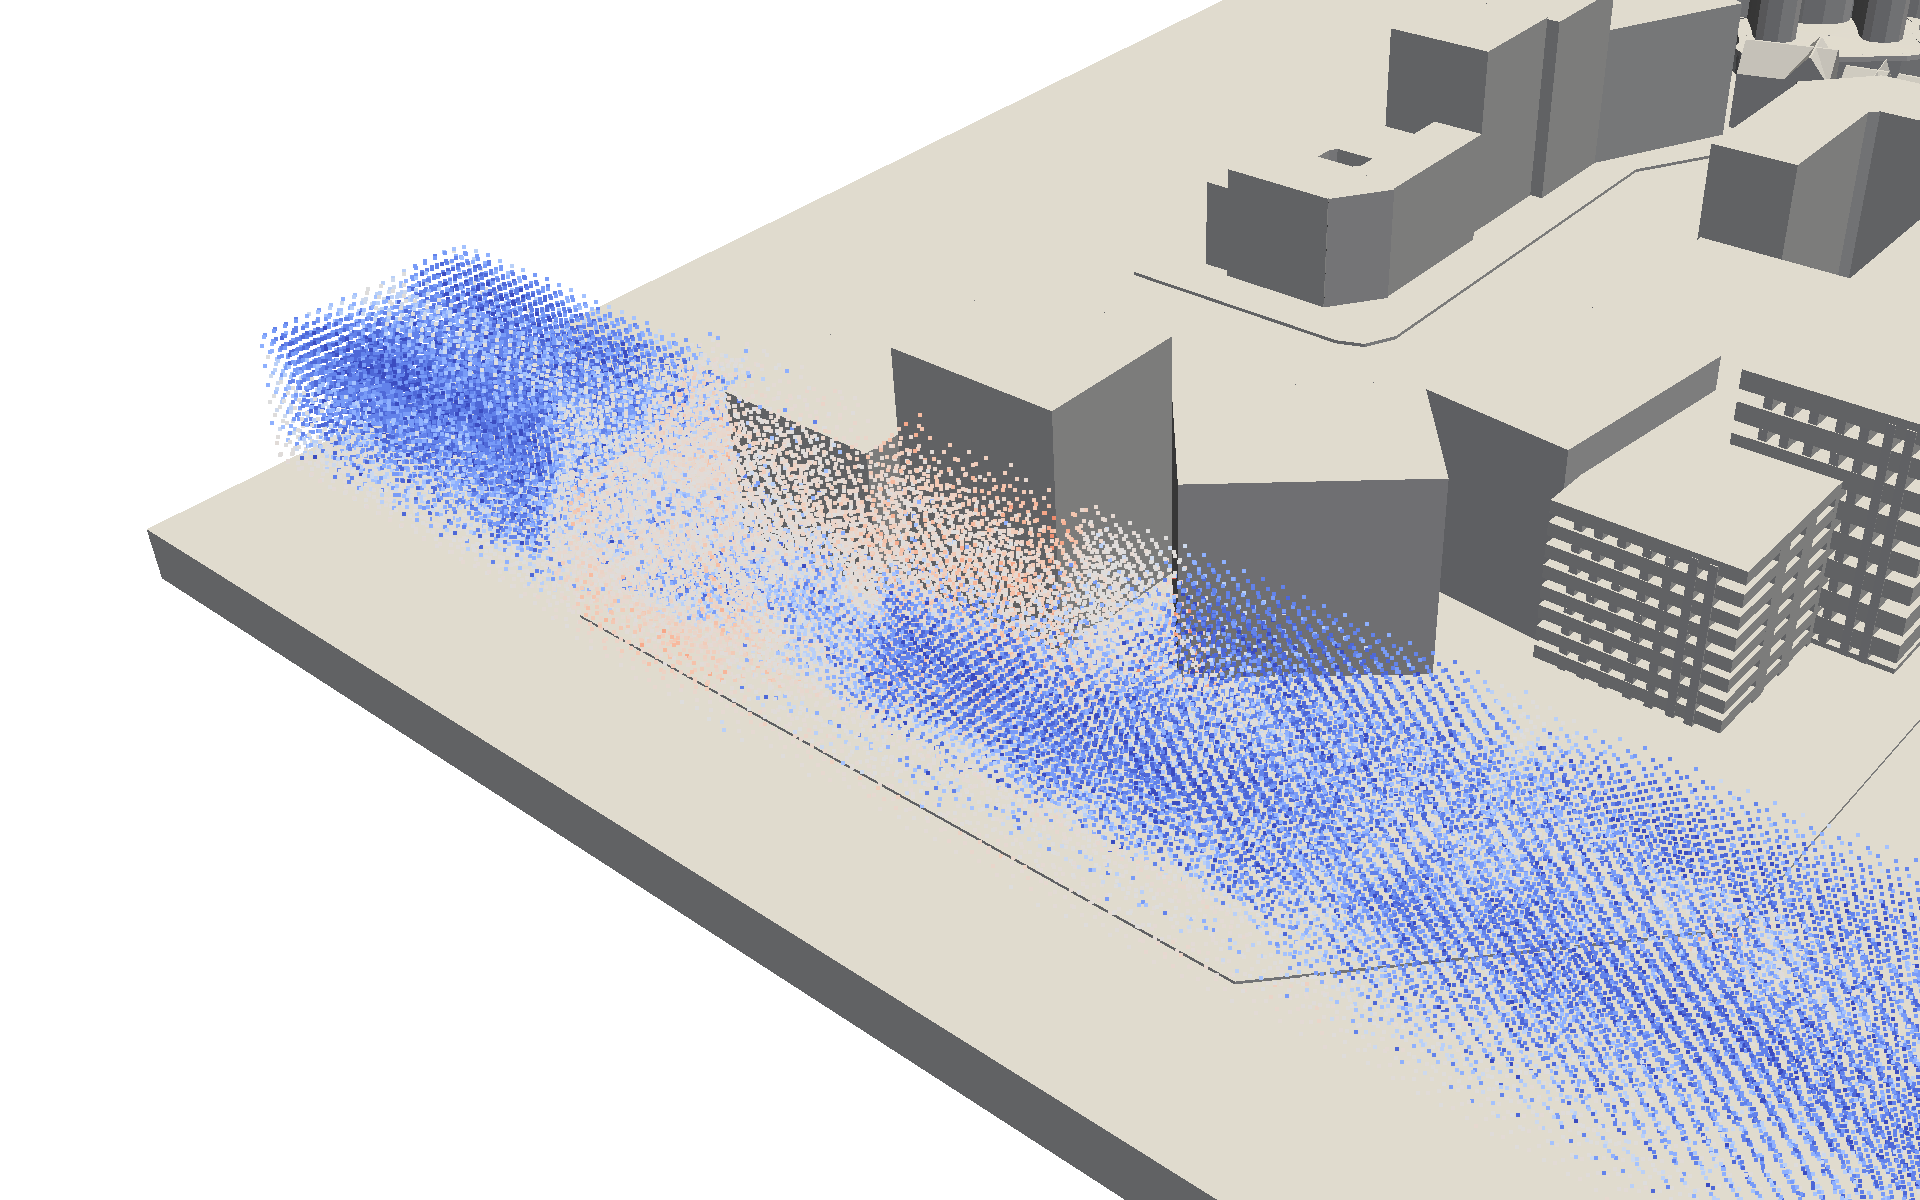
\includegraphics[width=\textwidth]{figures/visc-2.png}
  \end{subfigure}
  \begin{subfigure}{.5\textwidth}
    \centering
    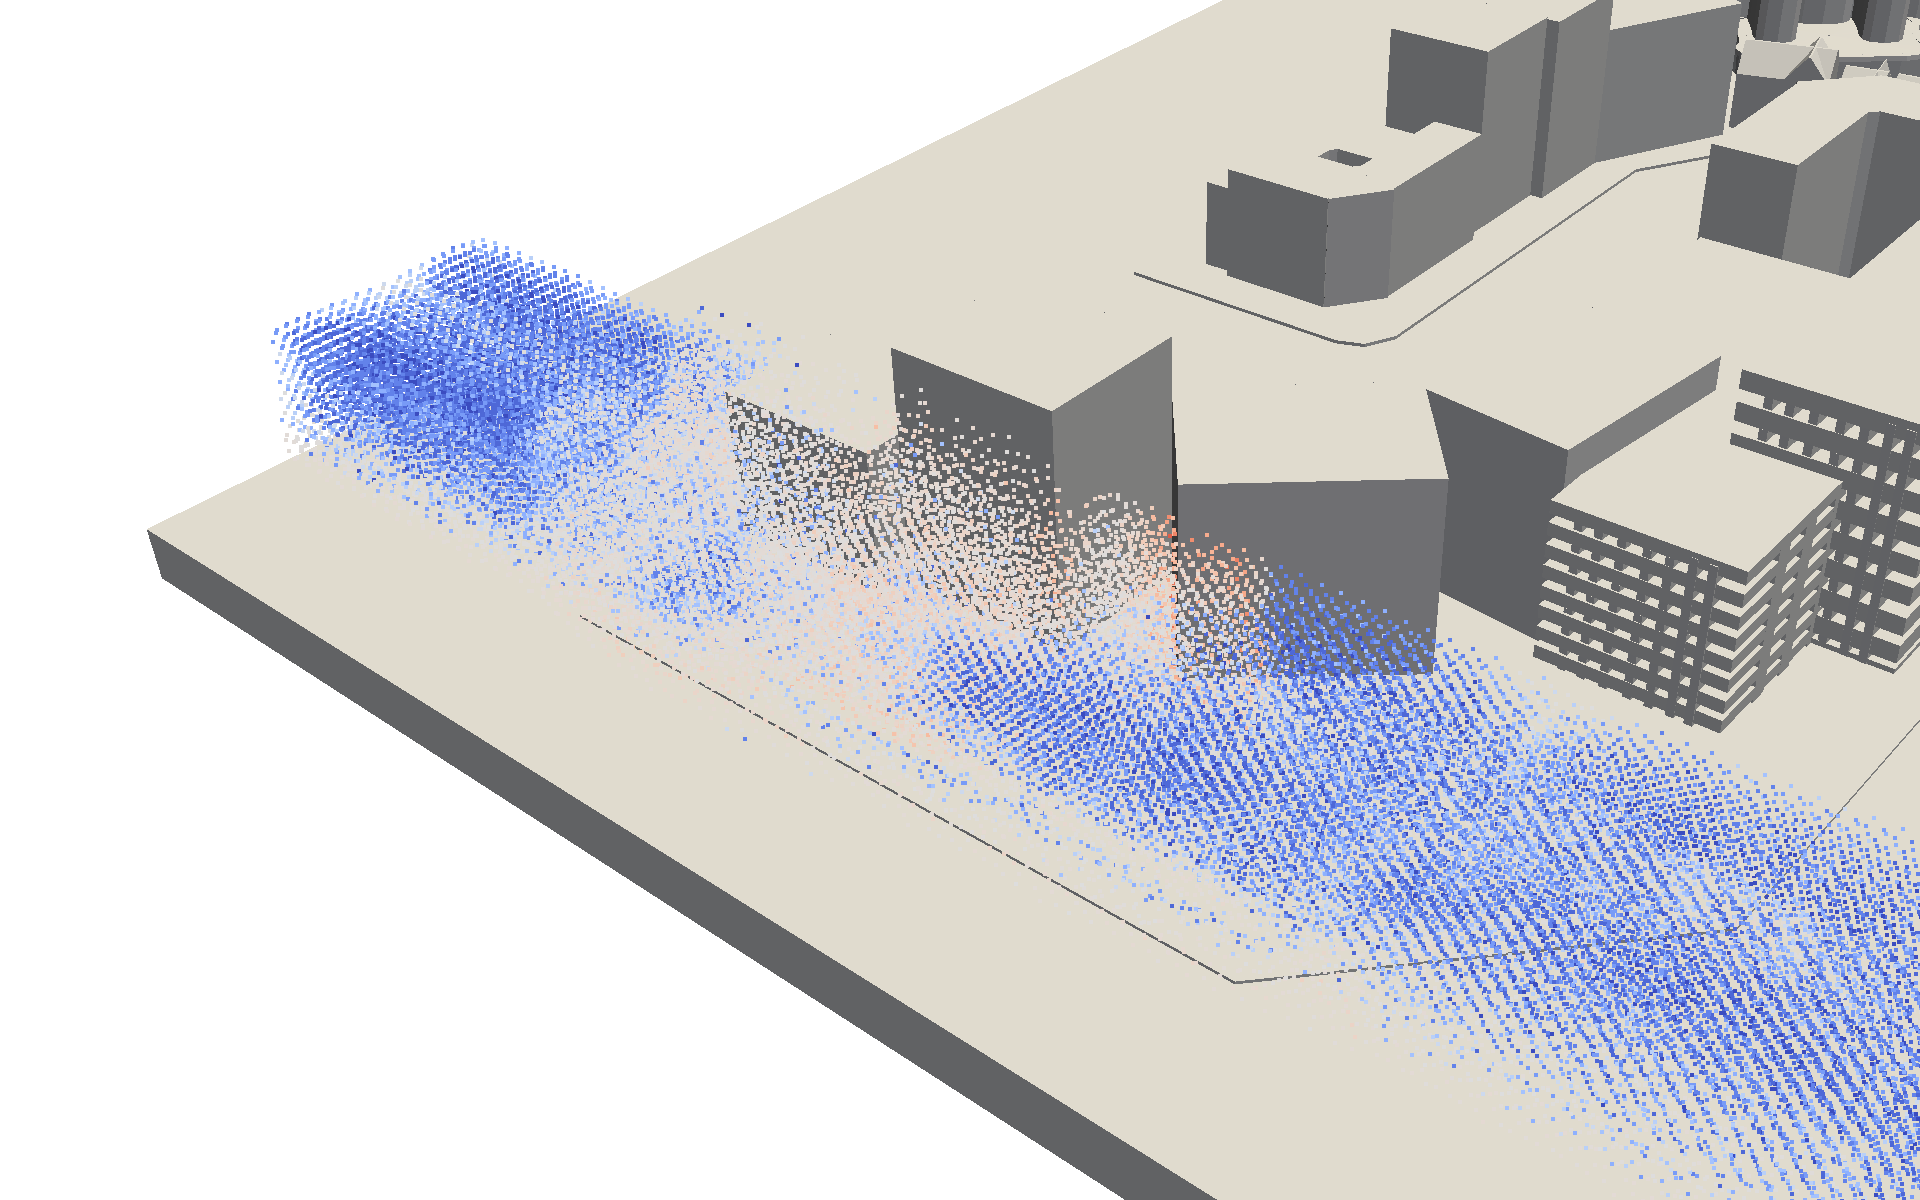
\includegraphics[width=\textwidth]{figures/visc-3.png}
  \end{subfigure}
  \caption[Δυνάμεις ιξώδους]{Διαδοχικά στιγμιότυπα προσομοίωσης όπου αποτυπώνεται
    χρωματικά στα σωματίδια το μέτρο της δύναμης που τους ασκείται λόγω ιξώδους του
    ρευστού. Η δύναμη του ιξώδους είναι ανάλογη της διαφοράς ταχύτητας μεταξύ γειτονικών
    σωματιδίων, και λόγω αυτού έχουν σημαντικό μέγεθος στις προσκρούσεις με εμπόδια,
    δεδομένης της απότομης αλλαγής ταχύτητας τμήματος του ρευστού (θερμότητα χρώματος
    ανάλογη του μέτρου της δύναμης).}
  \label{fig:viscosity-forces}
\end{sidewaysfigure}

\begin{sidewaysfigure}[]
  \centering
  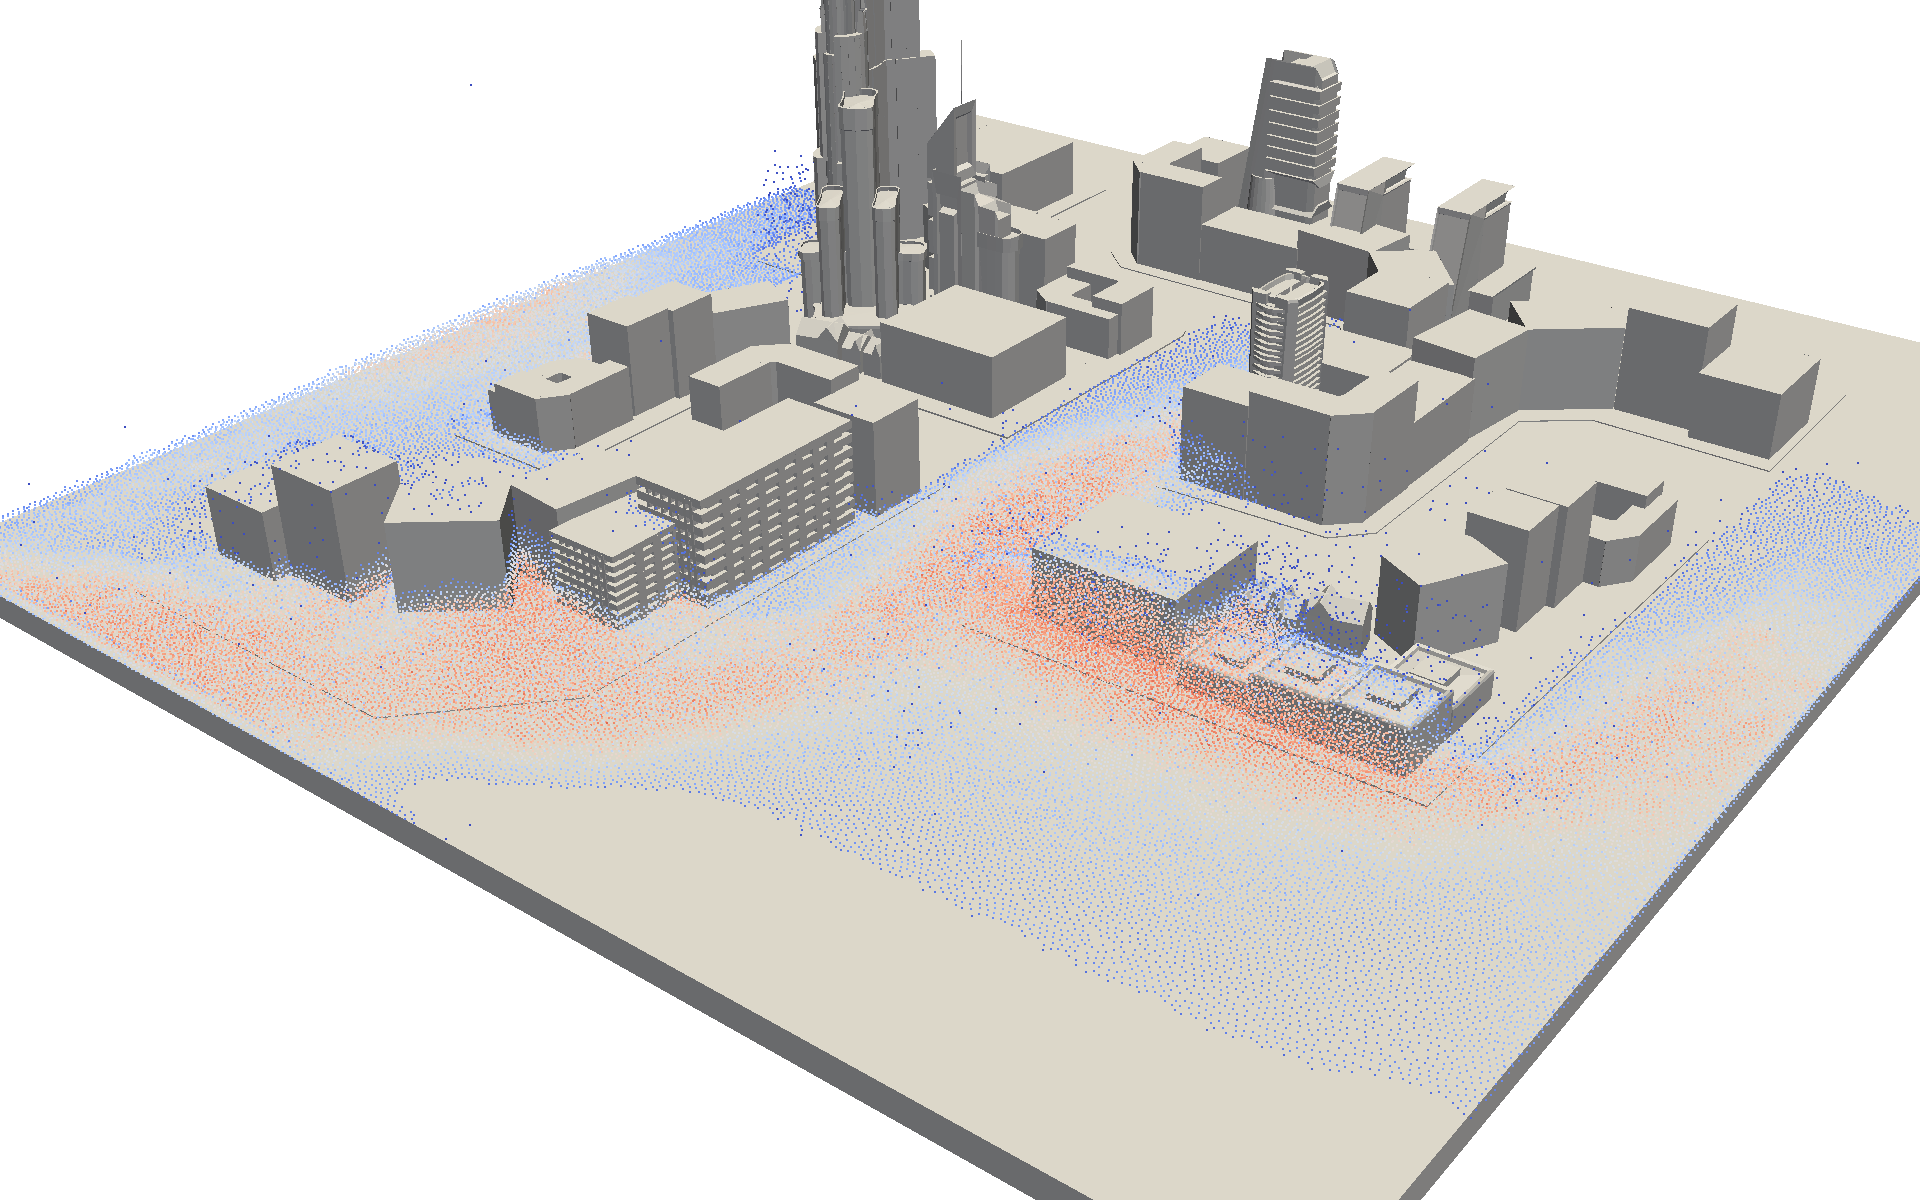
\includegraphics[width=\textwidth]{figures/samples.png}
  \caption[Απεικόνιση γειτονικών σωματιδίων] {Στιγμιότυπο προσομοίωσης όπου αναπαρίσταται
    χρωματικά ο αριθμός των δειγμάτων (γειτονικών σωματιδίων) που διατίθενται για την
    εκτίμηση των ιδιοτήτων του ρευστού (διακύμανση από σκούρο μπλε μέχρι έντονο κόκκινο, 0
    έως 52 δείγματα αντίστοιχα στην παρούσα περίπτωση). Λόγω της φύσης της προσομοίωσης
    (ροή σε ανοιχτό χώρο) είναι φανερή η έλλειψη ικανοποιητικού αριθμού δειγμάτων σε
    μεγάλο τμήμα του ρευστού, που οδήγησε και στην υιοθέτηση στοιχείων από \eng{PBD}
    (παράγραφος \ref{sssec:fluid-init}, \cite{Muller2007109, macklin2013position}).}
  \label{fig:samples}
\end{sidewaysfigure}

\begin{sidewaysfigure}[]
  \begin{subfigure}{.5\textwidth}
    \centering
    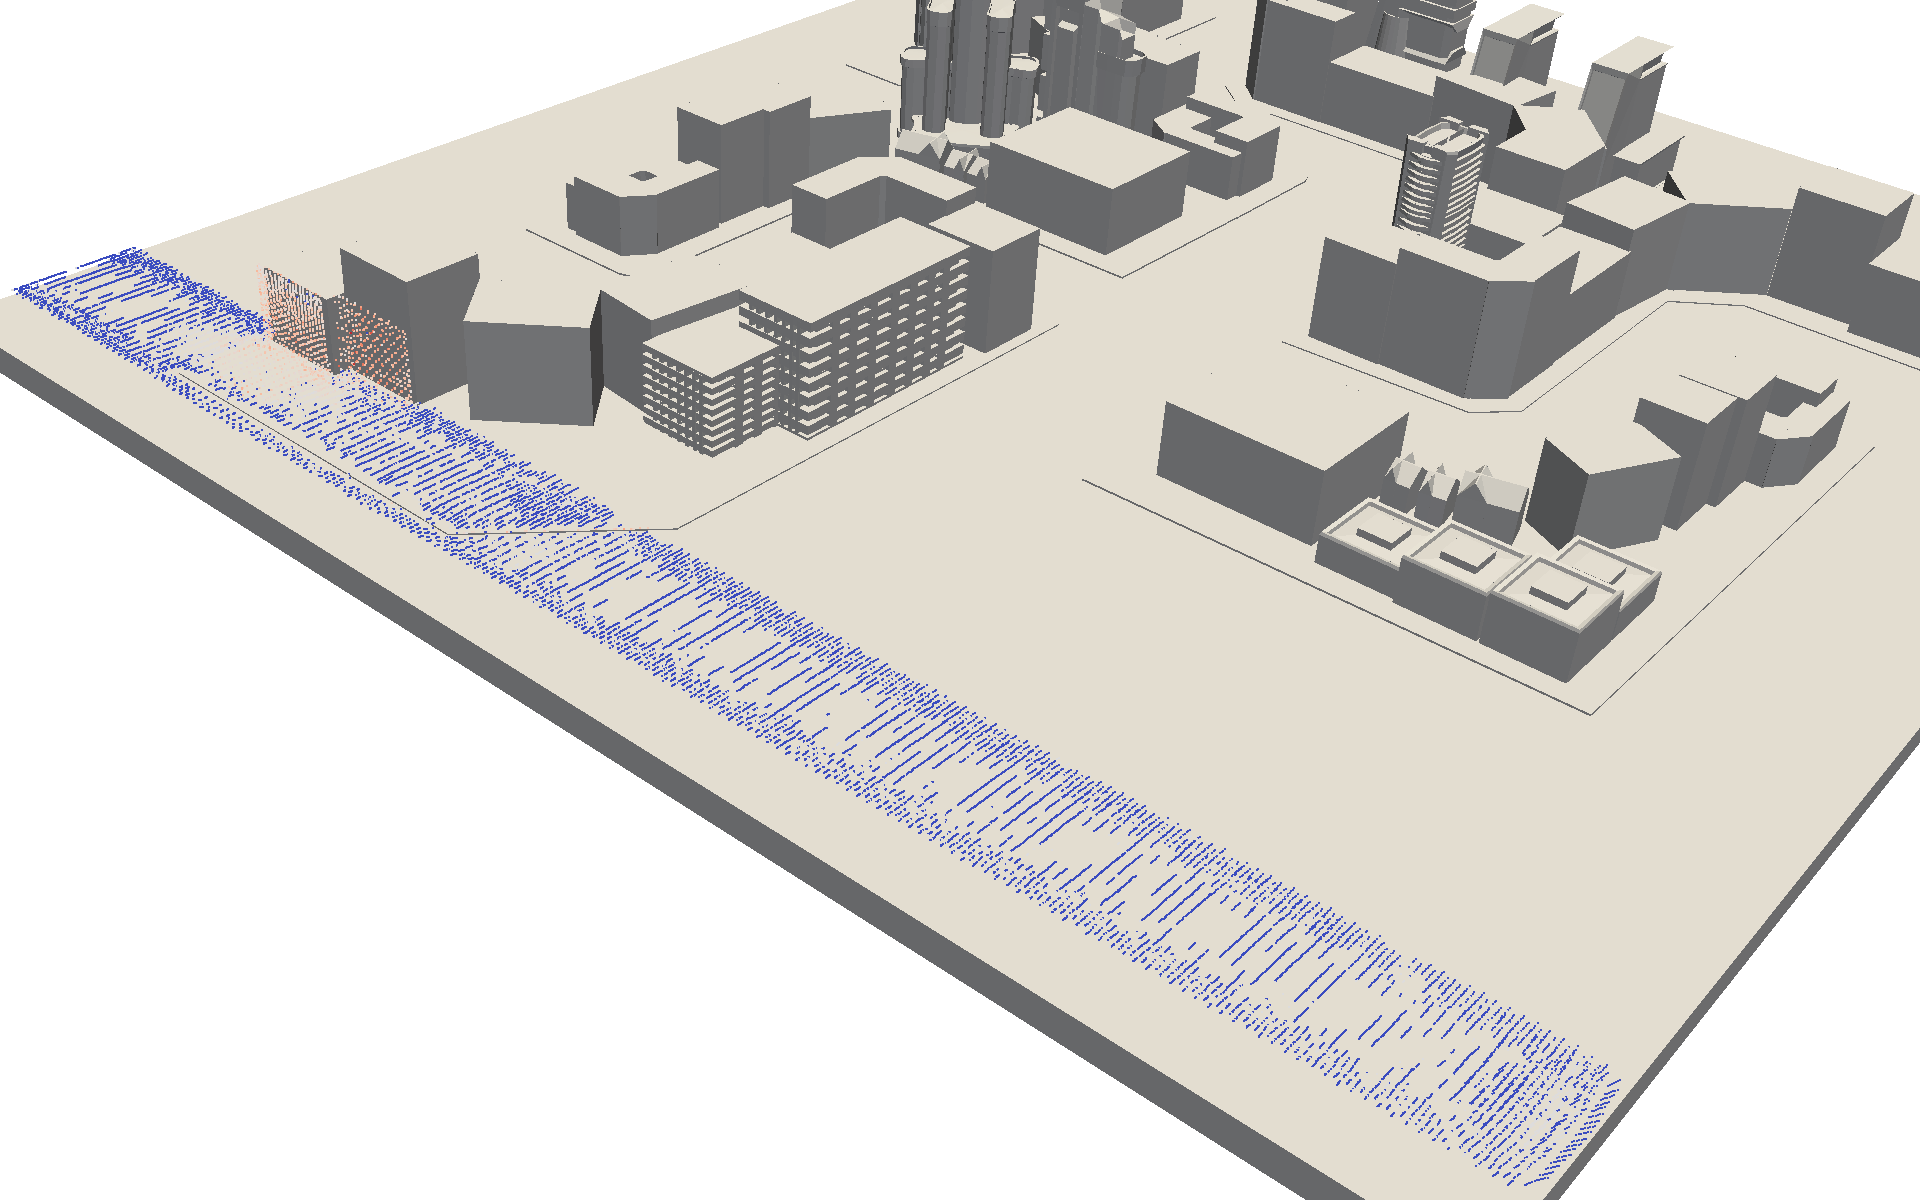
\includegraphics[width=\textwidth]{figures/impulses-0.png}
  \end{subfigure}
  \begin{subfigure}{.5\textwidth}
    \centering
    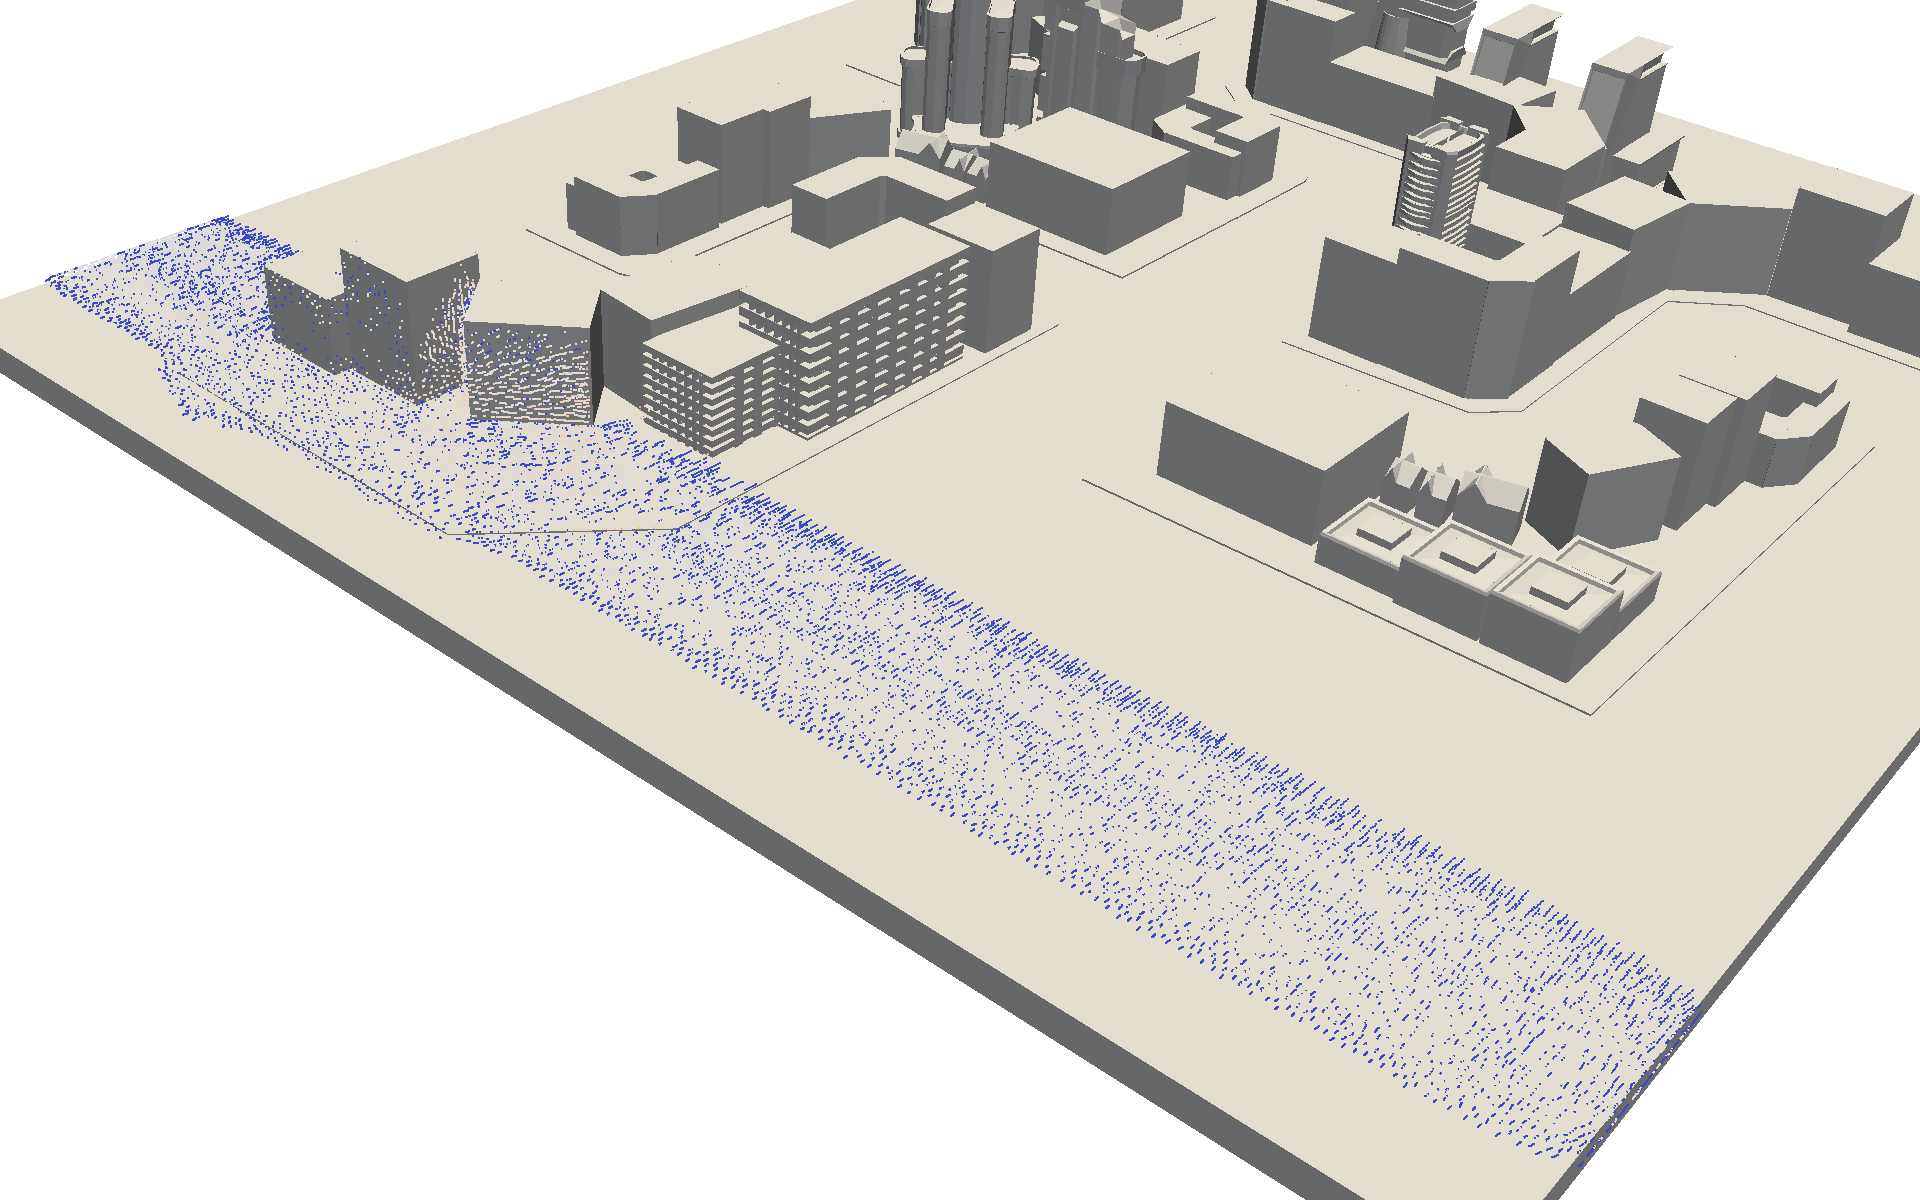
\includegraphics[width=\textwidth]{figures/impulses-1.png}
  \end{subfigure}
  \begin{subfigure}{.5\textwidth}
    \centering
    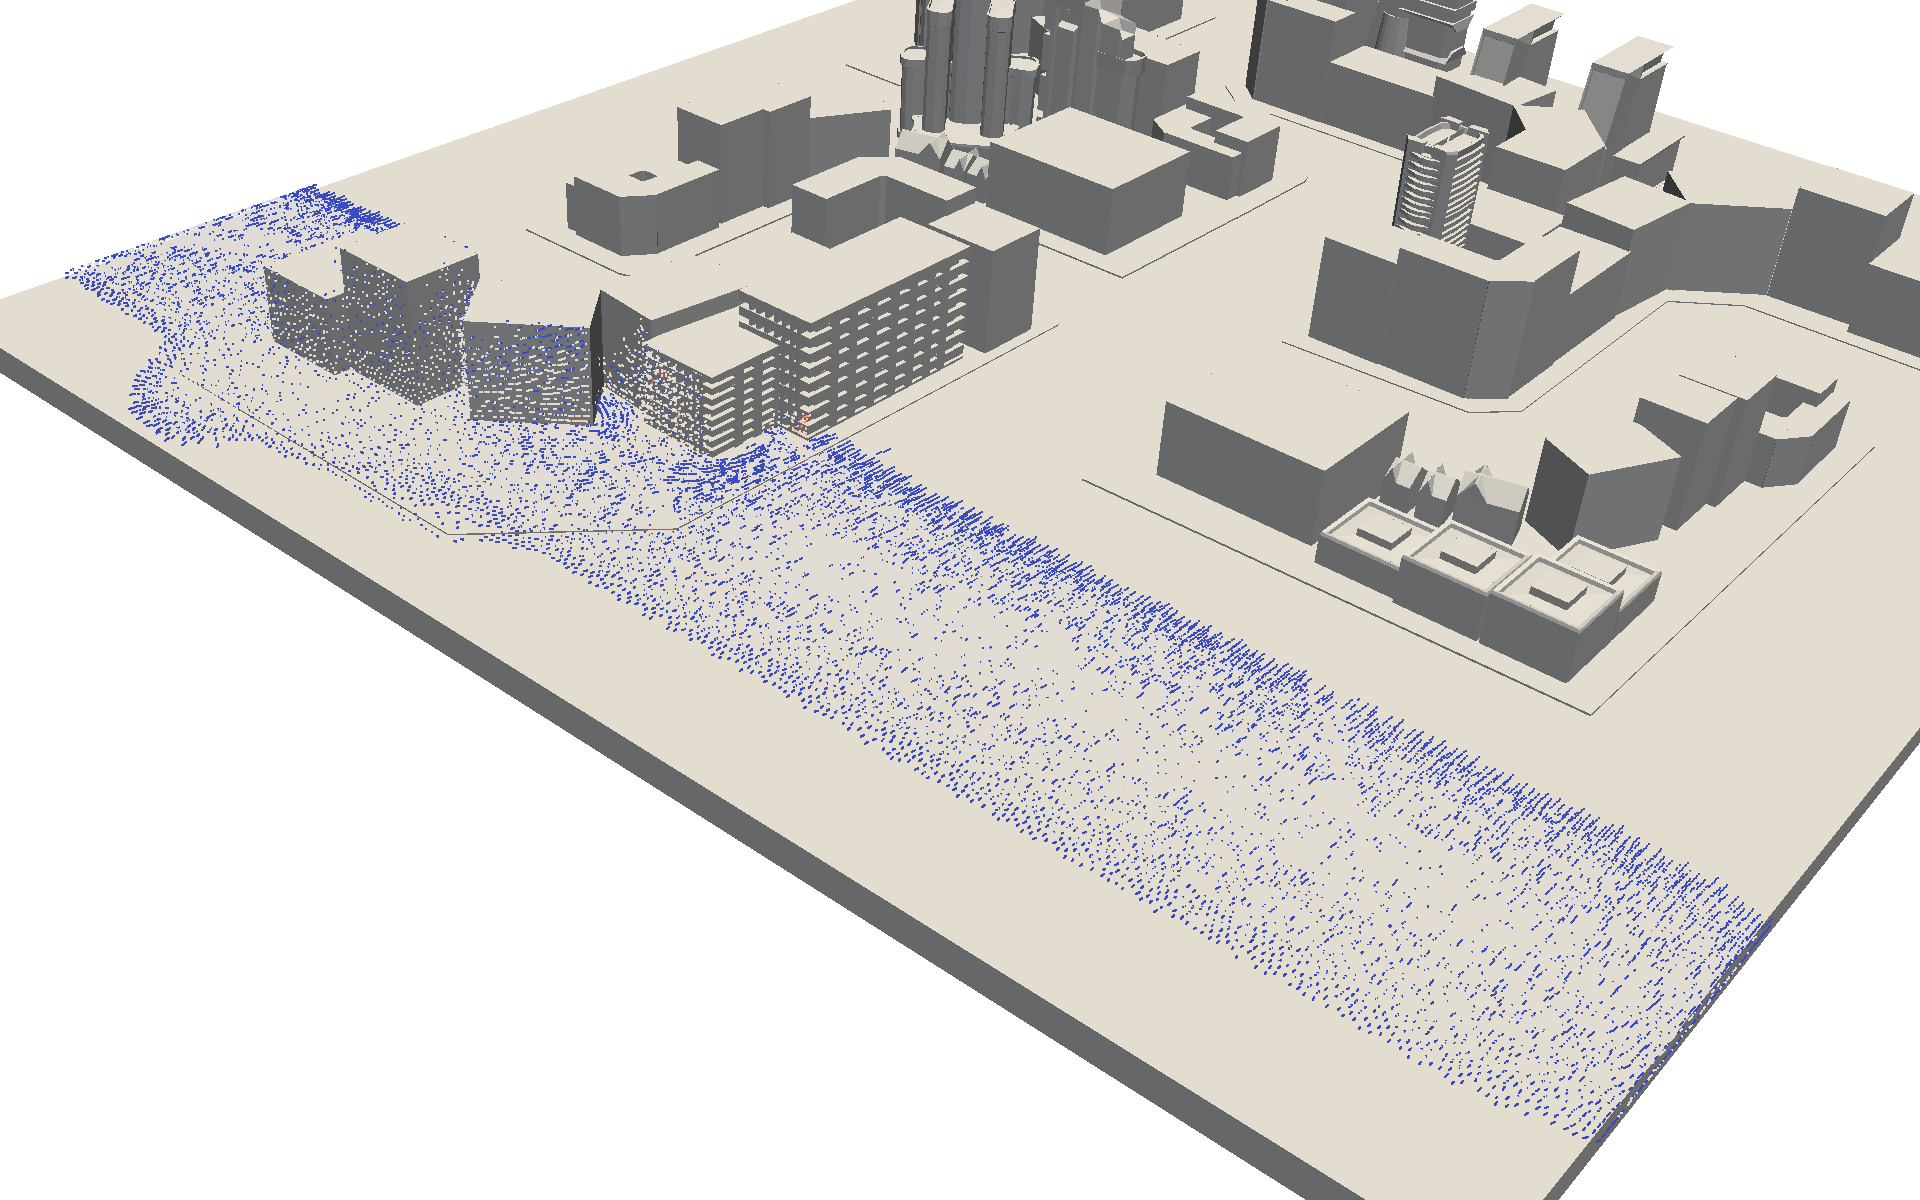
\includegraphics[width=\textwidth]{figures/impulses-2.png}
  \end{subfigure}
  \begin{subfigure}{.5\textwidth}
    \centering
    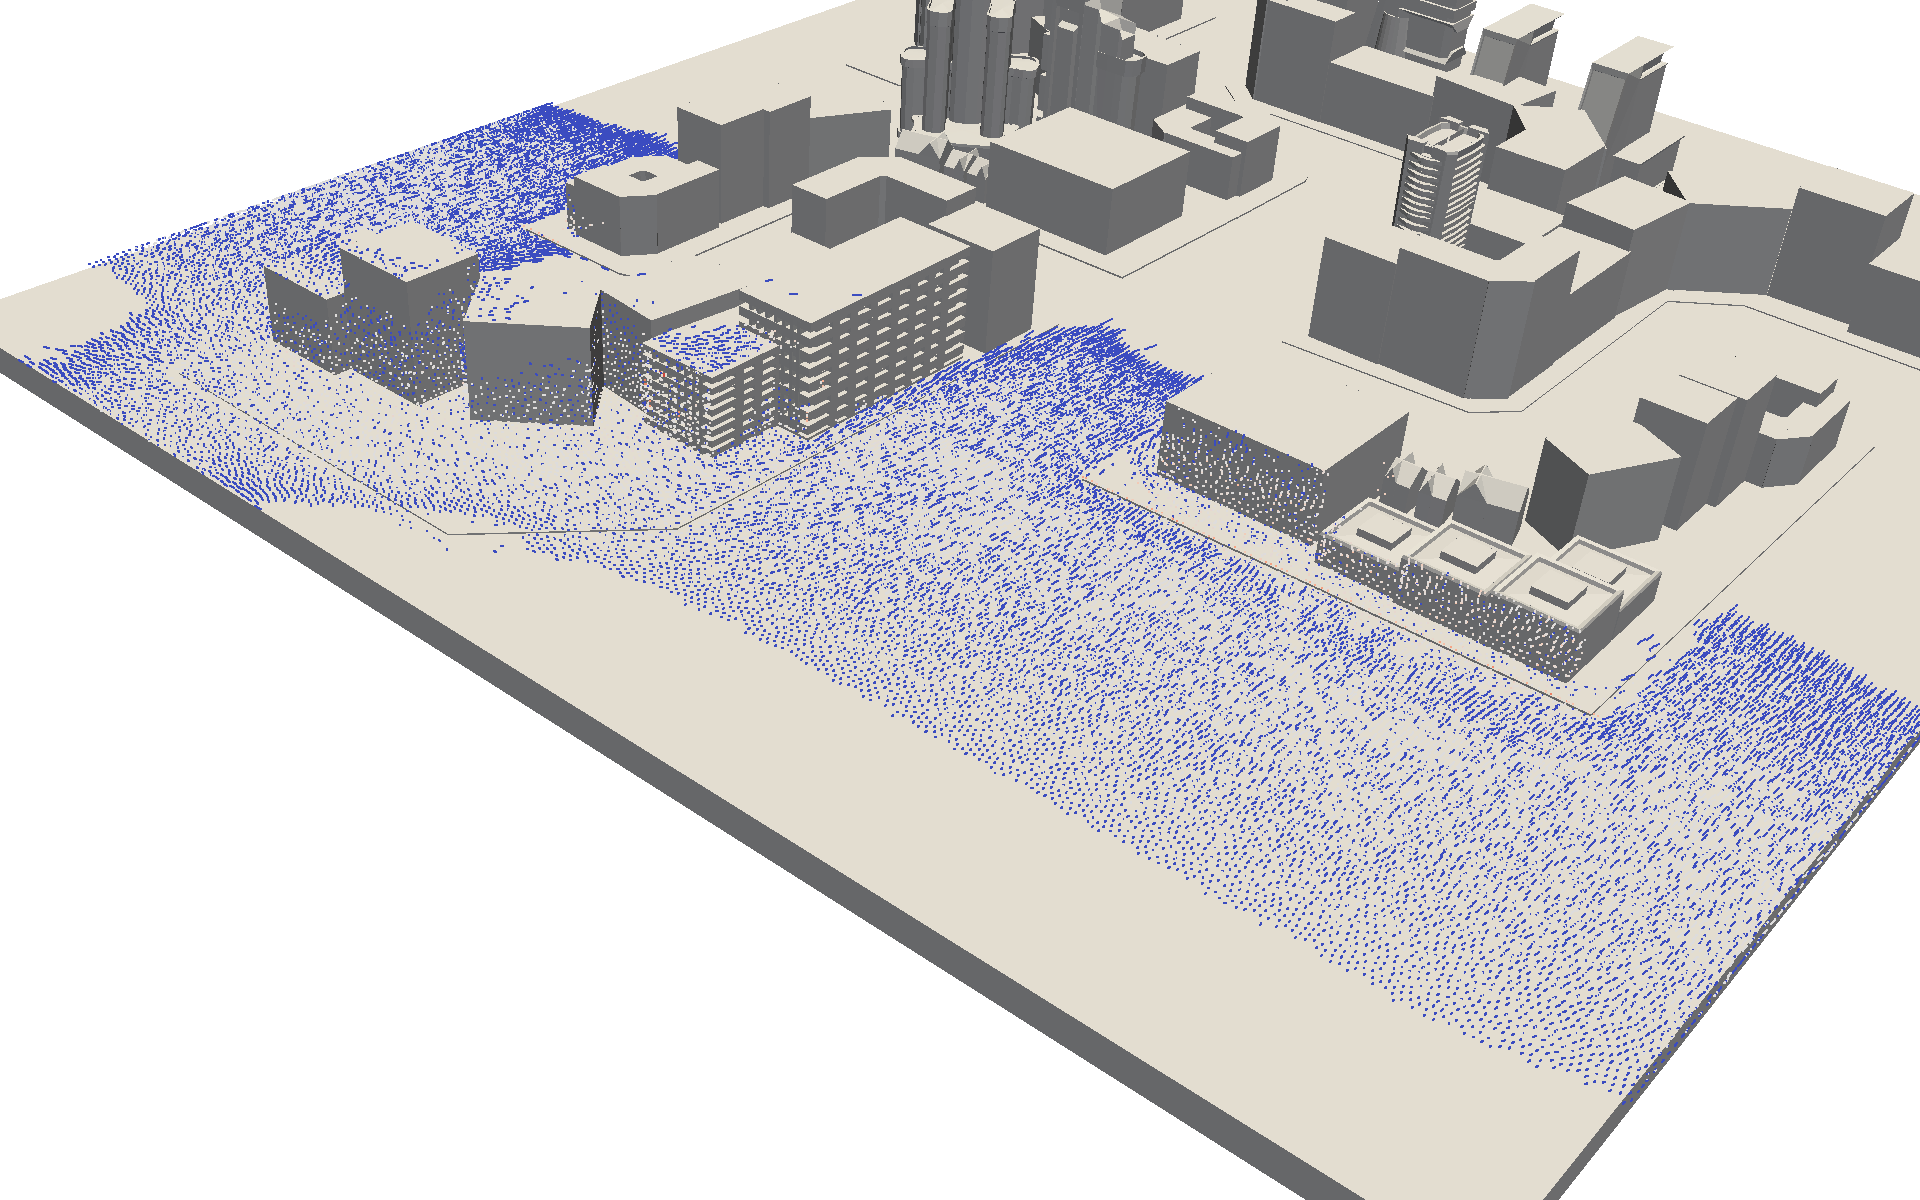
\includegraphics[width=\textwidth]{figures/impulses-3.png}
  \end{subfigure}
  \caption[Ώσεις στην ακτογραμμή]{Διάφορα στιγμιότυπα προσομοίωσης όπου αποτυπώνεται
    χρωματικά στην ακτογραμμή το μέτρο της ώσης που ασκείται από τα σωματίδια του ρευστού
    κατά την εξέλιξη του τσουνάμι (θερμότητα χρώματος ανάλογη του μέτρου της ώσης).}
  \label{fig:impulses}
\end{sidewaysfigure}

\subsection{Συμπεράσματα}
\paragraph{} Όπως φαίνεται στην εικόνα \ref{fig:impulse-fields}, έγιναν διάφορες
προσομοιώσεις πρόσπτωσης τσουνάμι έναντι αρκετών μοντέλων πόλεων, από τις οποίες
απεικονίζεται το \eng{heatmap} των ώσεων που ασκεί το κύμα στην ακτογραμμή, υπολογιζόμενο
αθροιστικά από όλες τις καταγραφόμενες ώσεις (παράγραφος \ref{sssec:simulation}). Όπως
εύκολα μπορεί να παρατηρηθεί, το μεγαλύτερο μέρος της ενέργειας του κύματος απορροφάται
από το πρώτο εμπόδιο που αυτό συναντά. Η παρατήρηση αυτή έρχεται σε πλήρη συμφωνία τόσο με
την εμπειρία από πραγματικά περιστατικά, όσο και από άλλες αναφορές στη
βιβλιογραφία. Χαρακτηριστικό παράδειγμα από πρόσφατο κρούσμα τσουνάμι αποτελεί το τσουνάμι
στον Ινδικό Ωκεανό στις 26 Δεκεμβρίου 2004, όπου περιοχές που προστατεύονταν κατά μήκος
της ακτογραμμής από δάση ριζοφόρων δέντρων (\eng{mangroves}) υπέστησαν πολύ μικρότερο
συγκριτικά πλήγμα \cite{danielsen2005asian, kathiresan2005601}, ενώ ποσοτικές προβλέψεις
που προέκυψαν από προσεγγιστικές θεωρητικές αναλύσεις του φαινομένου αυτού συμφωνούν με
μετρήσεις μεγεθών του κύματος, όπως του ύψους του \cite{yanagisawa200927}. Το γεγονός αυτό
έχει οδηγήσει στην κατασκευή τεράστιων κυματοθραυστών σε περιοχές με υψηλό κίνδυνο
πλήγματος από τσουνάμι. Παράδειγμα επιτυχούς αποτροπής σημαντικού πλήγματος αποτελεί η
πόλη \eng{Pondicherry} στην Ινδία, η οποία παρέμεινε σχεδόν άθικτη από το τεραστίου
μεγέθους παραπάνω τσουνάμι εξαιτίας του τεράστιου κυματοθραύστη που είχε κατασκευαστεί το
1735 από Γάλλους αποίκους και συνέχισε έκτοτε να συντηρείται. Ωστόσο οι κυματοθραύστες δεν
είναι πάντα αποτελεσματικοί. Η καταστροφή στο πυρηνικό εργοστάσιο \eng{Fukushima Daiichi}
το 2011 προκλήθηκε από το σεισμό και το ακόλουθο τσουνάμι της περιοχής \eng{Tōhoku} στην
Ιαπωνία, όταν τα κύματα ξεπέρασαν το ύψος των κυματοθραυστών που προστάτευαν τις
εγκαταστάσεις. Μεγάλη καταστροφή σημειώθηκε από το ίδιο τσουνάμι και στην περιοχή
\eng{Iwate}, παρά την εκτενή προστασία της από κυματοθραύστες συνολικού μήκους 25
\eng{km}, καθώς τα κύματα ξεπέρασαν σε ύψος πάνω από τους μισούς κυματοθραύστες. Οι
κυματοθραύστες απορροφούν το μεγαλύτερο ποσοστό της ενέργειας των κυμάτων, ωστόσο μεγάλο
μέρος της ζημιάς που προκαλείται από τσουνάμι οφείλεται στην πλημμύρα (\eng{flooding}) που
προκαλείται σε εκτεταμένες περιοχές της ακτογραμμής.

\paragraph{} Στην εικόνα \ref{fig:performance} απεικονίζεται ο μέσος χρόνος υπολογισμού
ενός στιγμιοτύπου \eng{frame} συναρτήσει του αριθμού σωματιδίων, υπολογισμένου από τα 10
πρώτα στιγμιότυπα προσομοιώσεων με 10\eng{k} έως 80\eng{k} σωματίδια, σχέση η οποία
φαίνεται να είναι τάξης $O(n log_2n)$ (συνεχής γραμμή). Λόγω των επιλεγμένων αρχικών
συνθηκών όπου τα σωματίδια βρίσκονται μόλις σε επαφή και στοιβαγμένα κατά το δυνατόν
συνεκτικότερα σε μικρό μέρος του τρισδιάστατου χώρου προσομοίωσης, τα πρώτα στιγμιότυπα
είναι κατά κανόνα αυτά με τον μεγαλύτερο υπολογιστικό φόρτο. Αν και οι συνθήκες αυτές δεν
επιτρέπουν την πλήρη συνεκτίμηση της επιτάχυνσης του προγράμματος από τη χρήση του \eng{LP
  grid} (δεδομένης της μη αξιοποίησης παρά μικρής έκτασης του πλέγματος), παρέχουν μια
αξιόπιστη εκτίμηση χειρότερης περίπτωσης (\eng{worst-case}) ανεξάρτητη από τη μορφολογία
της ακτογραμμής. Μία άλλη παράμετρος που πρέπει να σημειωθεί είναι οτι πυκνότερη
δειγματοληψία για τον ίδιο όγκο νερού συνεπάγεται μικρότερη ακτίνα σωματιδίων και αυτό με
τη σειρά του μικρότερο εσωτερικό χρονικό βήμα (σύμφωνα με τις παραγράφους
\ref{sssec:integration} και \ref{sssec:fluid-init}), άρα περισσότερα εσωτερικά βήματα
εντός ενός στιγμιοτύπου.

\paragraph{} Σε γενικές γραμμές η ποσοτική εκτίμηση της βελτίωσης στην ταχύτητα του
προγράμματος που επιτυγχάνεται με τη χρήση του \eng{LP grid} είναι δύσκολη, δεδομένου οτι
εξαρτάται από παραμέτρους της προσομοίωσης (αρχικές συνθήκες, δειγματοληψία, εσωτερική
αναπαράσταση σωματιδίων), μοτίβων πρόσβασης στα σωματίδια αλλά και του υλικού του
υπολογιστικού συστήματος (μεγέθος της κρυφής μνήμης). Τα αδιαμφισβήτητα πλεονεκτήματά του
περιλαμβάνουν:
\begin{itemize}
\item Συνεκτική αποθήκευση των σωματιδίων. Δεσμεύεται χώρος στη μνήμη ακριβώς ίσος με τον
  ελάχιστο δυνατό βάσει του μεγέθους της εσωτερικής αναπαράστασης των σωματιδίων.
\item Γρήγορη $Ο(1)$ πρόσβαση. Η ανάκτηση των σωματιδίων με βάση τη θέση τους γίνεται με
  λογική \eng{hash table} και είναι εγγυημένο οτι βρίσκονται όλα σε συνεχή περιοχή της
  μνήμης.
\item Ενημέρωση \eng{in-place}. Η ενημέρωση της δομής μετά από κάθε βήμα της προσομοίωσης
  δεν απαιτεί καμία επαναδεύσμευση (\eng{reallocation}) μνήμης και απαιτεί κατά κανόνα
  μικρό χρόνο (παράγραφος \ref{sssec:lp-grid-representation}).
\item Διατήρηση της τοπικότητας στην διάταξη αποθήκευσης. Τα σωματίδια κάθε κελιού είναι
  εγγυημένα αποθηκευμένα σε συνεχή περιοχή της μνήμης, ενώ σωματίδια γειτονικών κελιών
  βρίσκονται σε γειτονικές περιοχές της μνήμης, γεγονός που βελτιστοποιεί τη χρήση της
  κρυφής μνήμης σε υπολογισμούς αλληλεπιδράσεων εξαρτώμενων από την απόσταση στο χώρο.
\end{itemize}

\begin{figure}[]
  \begin{subfigure}{.5\textwidth}
    \centering
    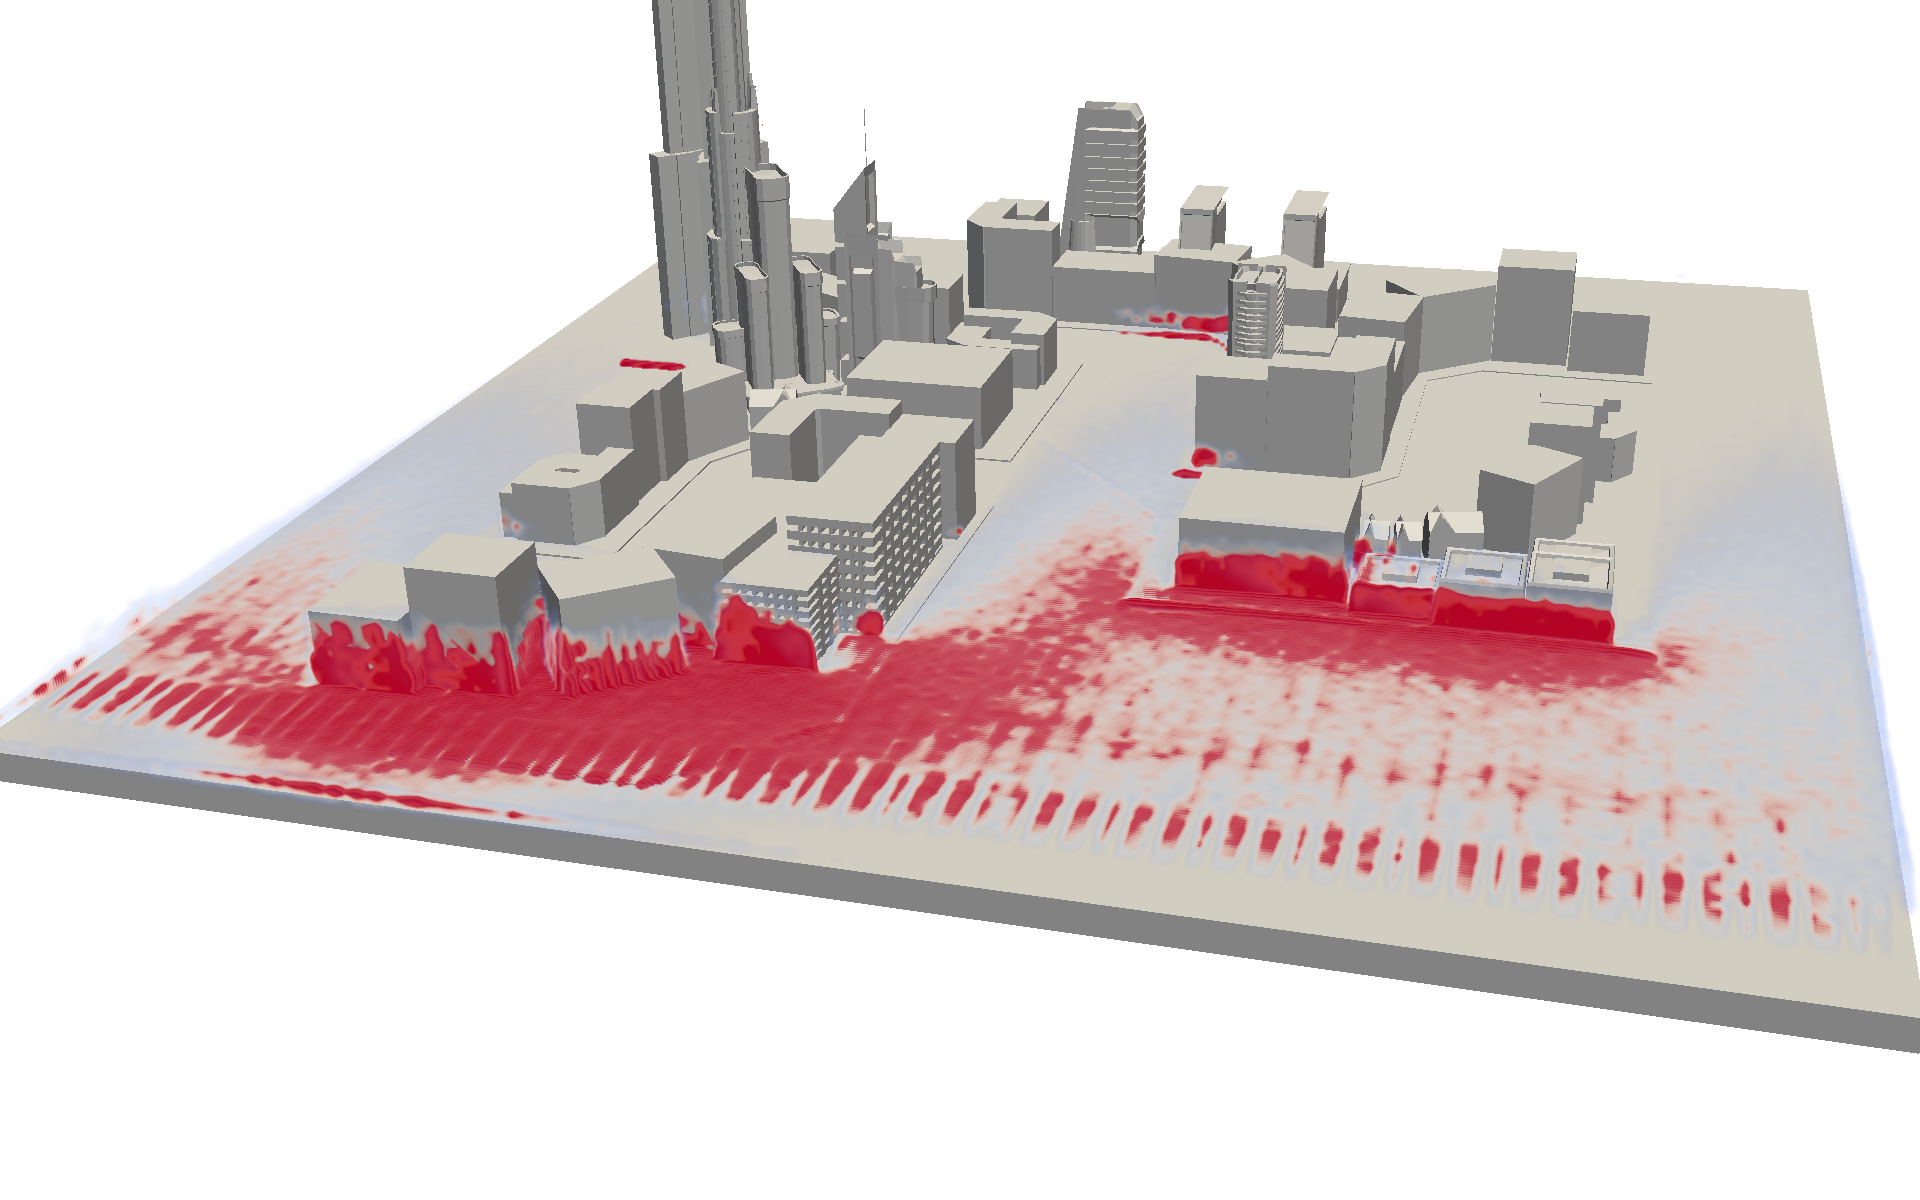
\includegraphics[width=\textwidth]{figures/impulse-heatmap-0.png}
  \end{subfigure}
  \begin{subfigure}{.5\textwidth}
    \centering
    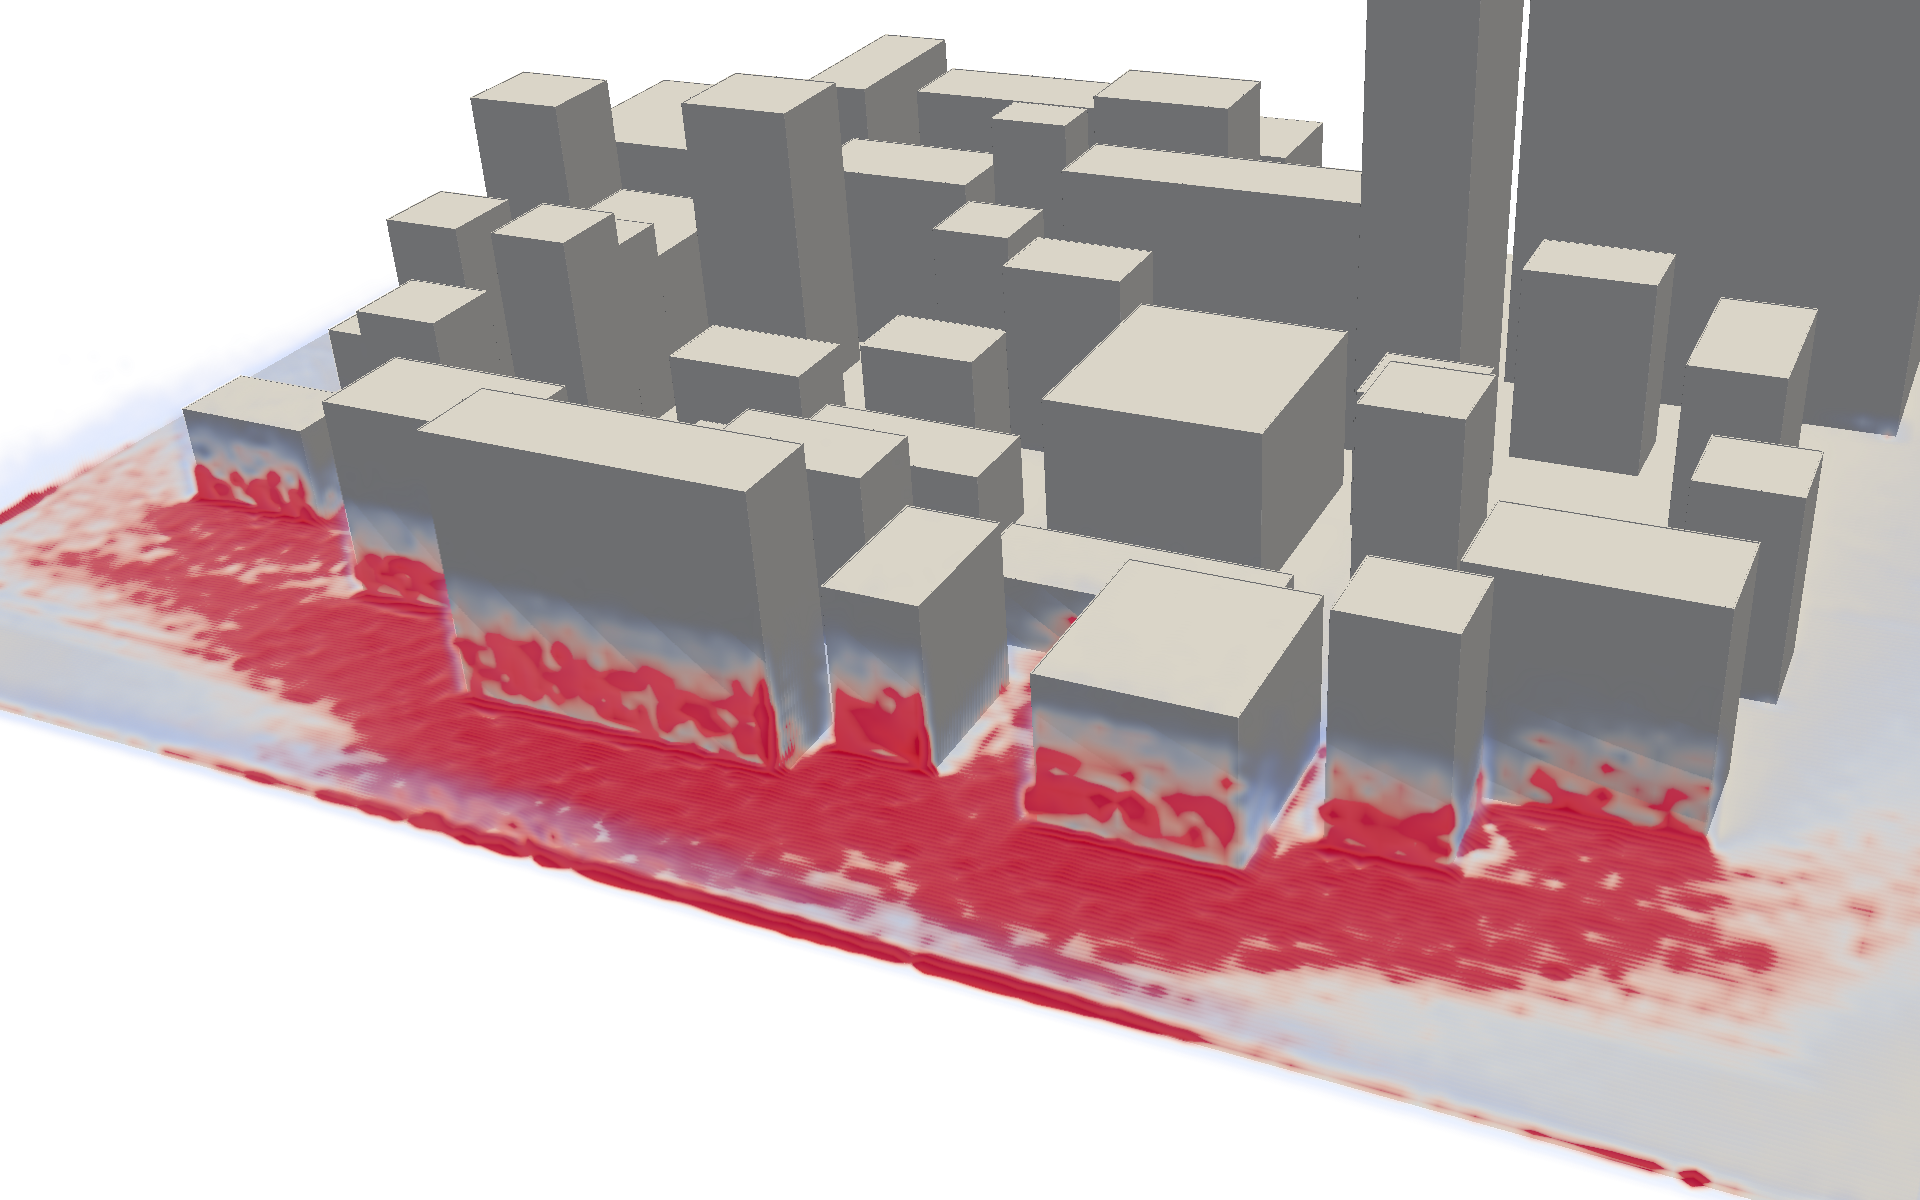
\includegraphics[width=\textwidth]{figures/impulse-heatmap-1.png}
  \end{subfigure}
  \begin{subfigure}{\textwidth}
    \centering
    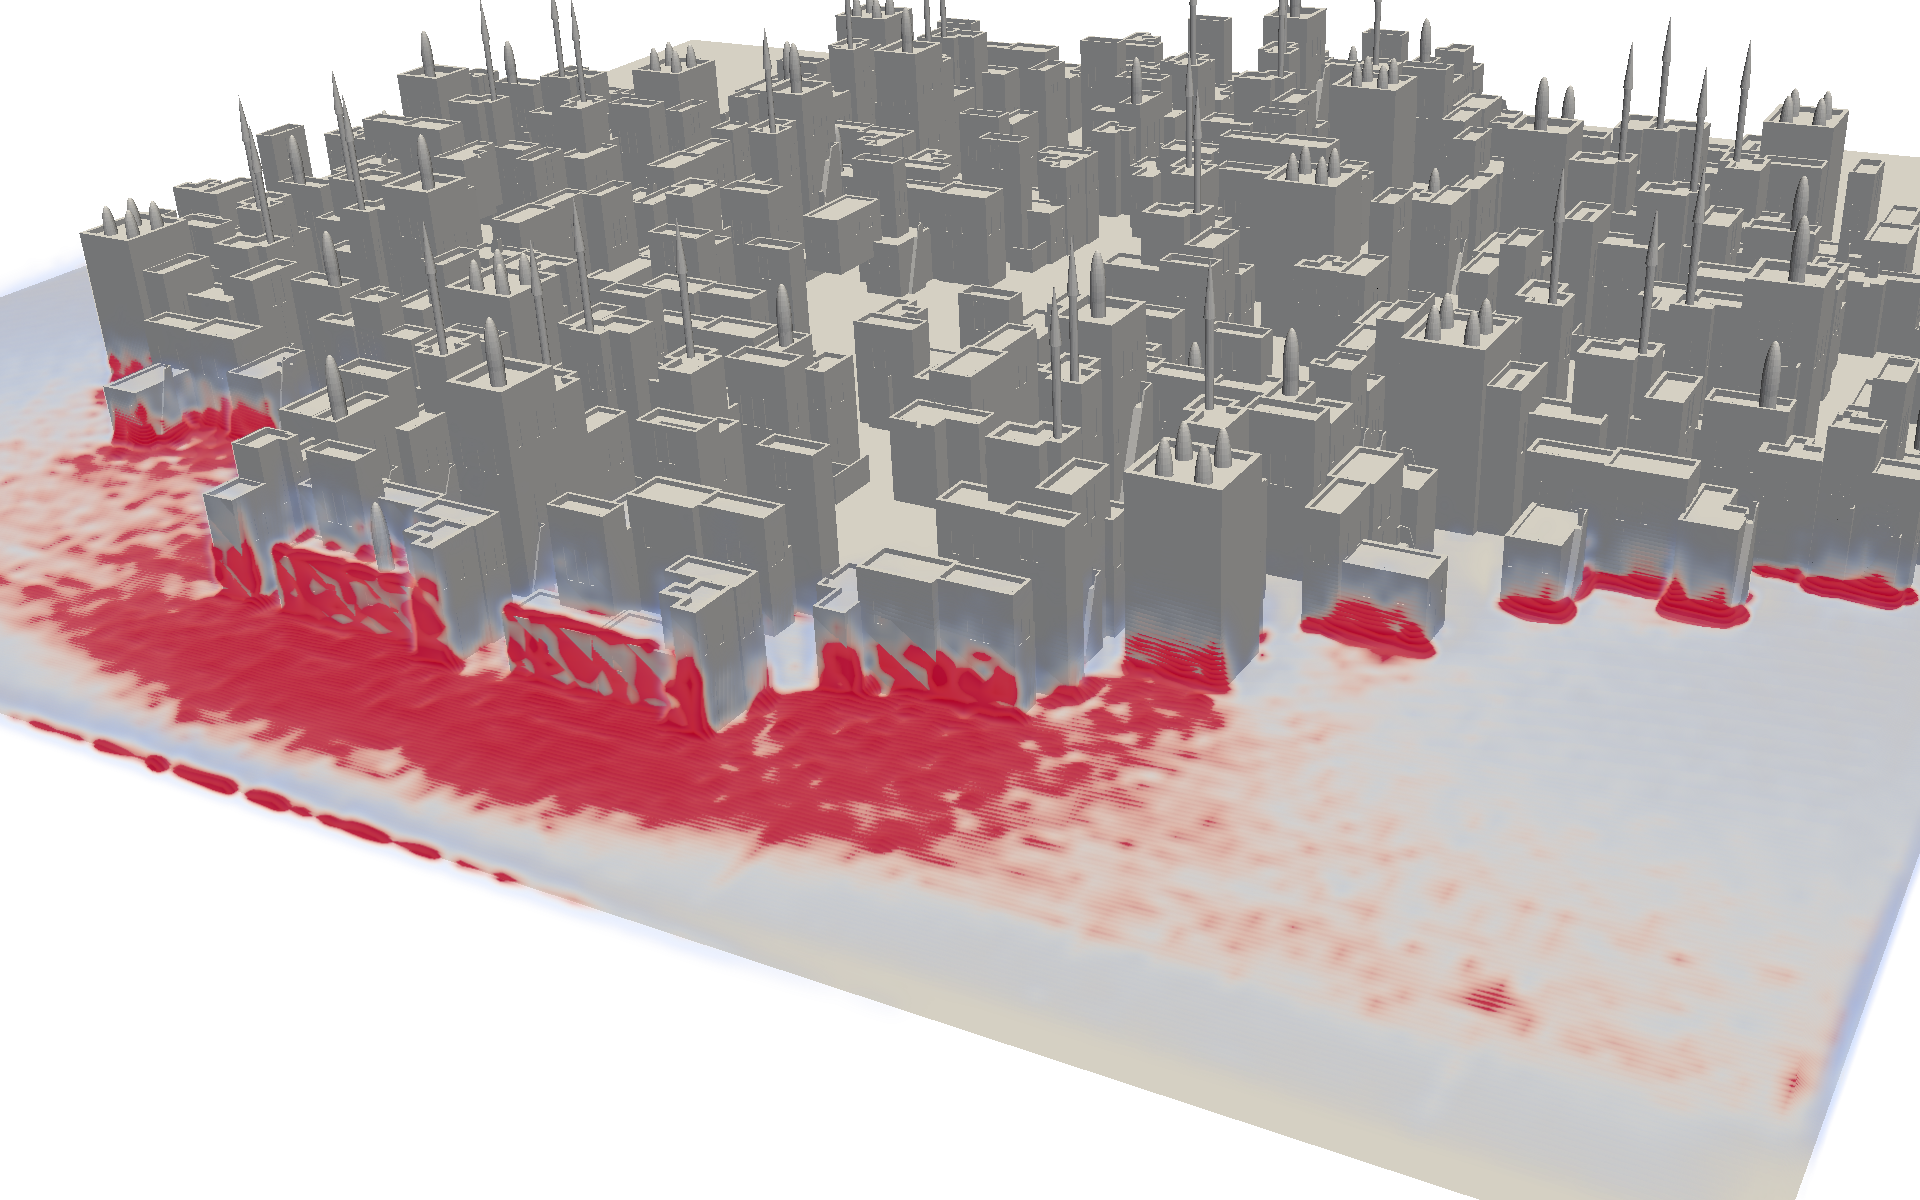
\includegraphics[width=\textwidth]{figures/impulse-heatmap-2.png}
  \end{subfigure}
  \caption[\eng{Heatmap} ώσεων στην ακτογραμμή]{\eng{Heatmap} των ώσεων του ρευστού προς
    την ακτογραμμή καθ' όλη την εξέλιξη του κύματος, σε τρία διαφορετικά μοντέλα
    πόλης. Επιβεβαιώνεται οτι το μεγαλύτερο μέρος της ενέργειας του κύματος απορροφάται
    από από τα πρώτα εμπόδια που αυτό συναντά, φαινόμενο που έχει δειχθεί τόσο σε
    καταγραφές πραγματικών περιστατικών, όσο και στη βιβλιογραφία.}
  \label{fig:impulse-fields}
\end{figure}

\begin{figure}[]
  \centering
  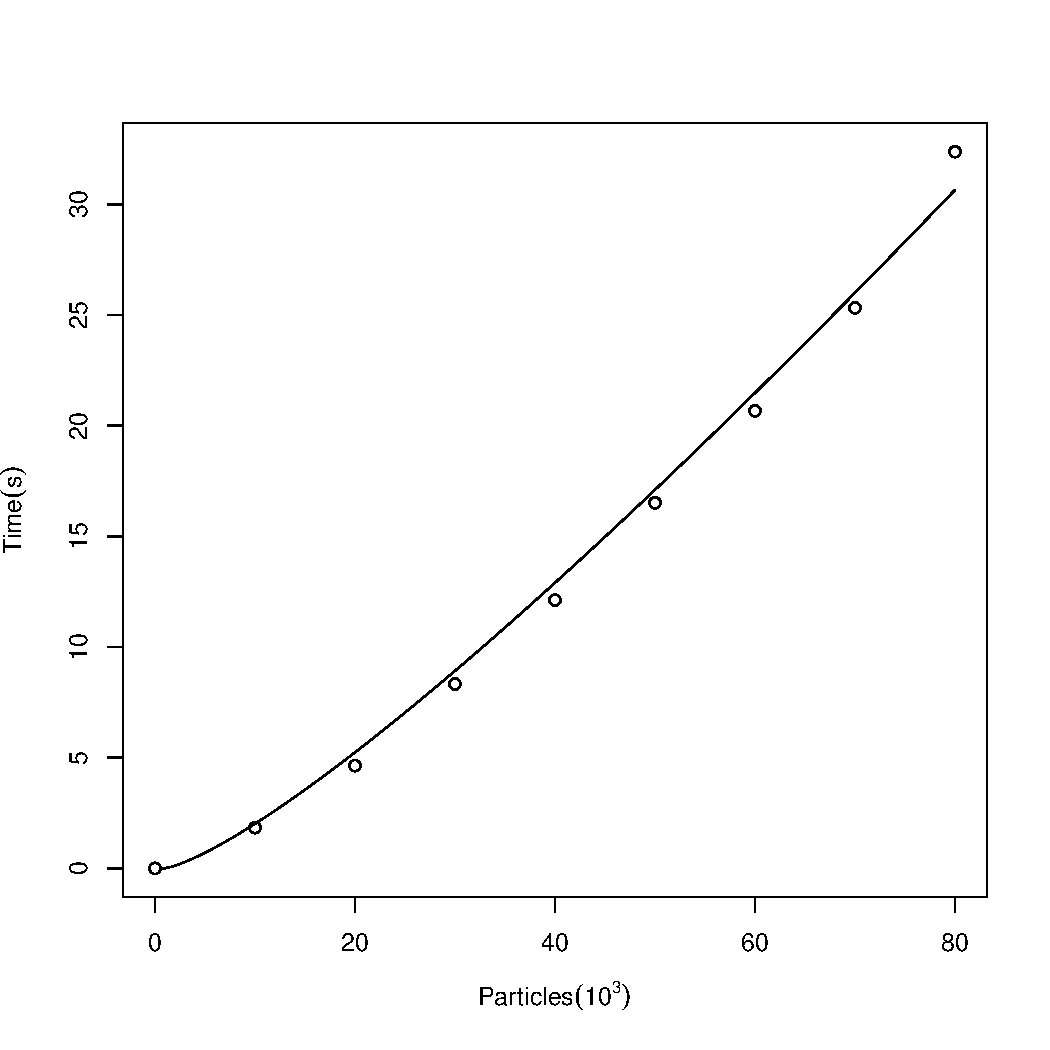
\includegraphics[width=\textwidth]{figures/performance.pdf}
  \caption[Απόδοση προγράμματος προσομοίωσης] {Γραφική παράσταση του μέσου χρόνου
    υπολογισμού ενός στιγμιοτύπου \eng{frame} συναρτήσει του αριθμού σωματιδίων,
    υπολογισμένου από τα 10 πρώτα στιγμιότυπα προσομοιώσεων με 10\eng{k} έως 80\eng{k}
    σωματίδια (η συνεχής γραμμή αναπαριστά $Ο(n log_2n)$ αύ\-ξη\-ση). Περίπου τα 3/4 του
    χρόνου εκτέλεσης αντιστοιχούν σε διεργασίες της \eng{Bullet} και καταγραφής δεδομένων
    εξόδου, ενώ το 1/4 σε διεργασίες της μηχανής \eng{SPH} που αναπτύχθηκε.}
  \label{fig:performance}
\end{figure}

%%% Local Variables:
%%% mode: latex
%%% TeX-master: "report"
%%% End:

% \clearpage
% \input{discussion.tex}
\clearpage
\selectlanguage{english} %\footnotesize
\renewcommand{\refname}{\gre{Βιβλιογραφία}}
\bibliographystyle{acm}
\bibliography{bibliography} 
\selectlanguage{greek} \normalsize

\end{document}

%%% Local Variables: 
%%% mode: latex
%%% TeX-master: t
%%% End: 
